\documentclass[11pt]{article}

\usepackage[utf8]{inputenc}
\usepackage{geometry}
\usepackage{setspace}
\usepackage{parskip}
\usepackage{amsmath}
\usepackage{amssymb}
\usepackage{enumitem}
\usepackage{hyperref}
\usepackage{graphicx}
\usepackage{float}
\usepackage{caption}
\usepackage{natbib}
\usepackage{longtable}
\usepackage{booktabs}
\usepackage{array}
\usepackage{placeins}
\usepackage{xcolor}
\usepackage{soul}
\usepackage{todonotes}

\geometry{margin=1in}
\onehalfspacing

\begin{document}

% =========================================================
% TITLE PAGE
% =========================================================
\begin{titlepage}
    \centering

    \vspace*{1.3in}

    {\Large\scshape Generative Sabermetrics \par}

    \vspace{0.85in}

    {\Huge\bfseries Generative Sabermetrics:\\[0.25em]
    A Physics-Based Simulation Framework for Baseball Intelligence\par}

    \vspace{0.75in}

    \rule{0.72\textwidth}{0.4pt}

    \vspace{0.45in}

    {\large
    Evan Goforth
    \par}

    \vspace{0.35in}

    {\large May 21, 2026 \par}

    \vfill

    {\small
    Generative Sabermetrics
    \par}

\end{titlepage}

\newpage

\section{Introduction}

In recent years, many physical sciences such as biology, chemistry, and physics have benefited from advancements within the machine learning community. The intersection of science and machine learning has given rise to an interdisciplinary field aptly named Scientific Machine Learning (SciML). 
SciML utilizes prior domain knowledge and physical structure, philosophically similar to informed priors within Bayesian methods, to constrain machine learning architectures to ensure learned patterns and relationships are within the grounds of physical plausibility. In contrast to purely data-driven modeling, SciML is especially useful when the target process is partially observed but constrained by known physical relationships.\citep{karniadakis2021physicsinformed, willard2022integrating, karpatne2017theoryguided}.

This criteria is present within the game of baseball due to the physics that underlie the game. The spin and speed of the baseball dictate the movement of each pitch, which is then struck with a wooden bat where normal and tangential forces redirect the ball into the field of play. The bat--ball collision has a substantial physics literature, including rigid-body and flexible-bat collision models, normal and tangential restitution, and oblique collision behavior \citep{cross1999impact, nathan2000dynamics, nathan2003characterizing, cross2006scattering, kensrud2017oblique}. 

Modern tracking systems such as Statcast provide observed pitch and batted-ball measurements \footnote{We used the PyBaseball Statcast pitch level dataset for our study} which encapsulate almost all of the physically relevant aspects of a single pitch realization. The first part of this study, using the philosophies of SciML, combines the aforementioned physical constraints known from the bat-ball collision process literature with the PyBaseabll Statcast data set to infer critical, yet unobserved, variables. The result of this inference is an augmented dataset which includes nearly all physically relevant variables to the bat-ball collision process. This augmented dataset is then used to model the \hl{data-generating mechanism} \footnote{The data-generating mechanism refers to the unobserved forces at play which dictates how realizations of a given process or system are produced} of the bat-ball collision process. We believe this framework could lead to exciting new directions in sabermetrics and deepening the understanding of baseball at it's most granular level.\citep{kagan2017Statcast}. 

The current state of sabermetrics and baseball modeling primarily works within a predictive or descriptive modeling paradigm. Descriptive statistics aims to aggregate many events over long periods of time into summary statistics which can be quite useful as heuristics. Predictive modeling aims to capture patterns and \hl{correlations} within data, where a given context (input), is mapped to a predicted outcome (output). Predictive modeling has been very successful in sports analytics, especially in the data heavy baseball realm. Prior academic applications of machine learning in baseball have largely focused on task-specific prediction problems, including pitch-type prediction, pitch-location prediction, game-outcome prediction, and pitch-outcome or swing-decision modeling \citep{hamilton2014applying, hoang2015dynamic, sidle2018using, lee2022prediction, yu2022decide, huang2021use, gopal2024baseball}.

A newer form of modeling has been gaining traction in many applications: Generative modeling. \hl{Generative and simulation-based approaches seek to represent a conditional data-generating process} \citep{cranmer2020frontier,deistler2025simulation}. In this sense, a generative model is not limited to predicting a target variable, but learns a distribution which can simulate synthetic data: New realizations of the underlying process under specified contextual and physical assumptions. Additionally, generative models allow for individual components of the process to be \hl{intervened} upon while other components are held fixed. The second goal of this study was to utilize our comprehensive, augmented dataset to train, calibrate, and test generative model architectures such that they would be able to learn the data-generating mechanism of the bat-ball collision process.

Recent academic work has begun to frame baseball explicitly as a generative, world-modeling problem. Most notably, \citet{ahn2026neural} serialize play-by-play tracking data into token sequences and train an LLM-based world model for pitch-level prediction. Their approach models baseball as an autoregressive event sequence and does a great job at predicting discrete state space events including pitch selection and swing decision. The study explicitly states that more work must be done to explore the baseball world model component to include batted-ball trajectory. Our study looks to build upon Ahn et.al's baseball world model to also encapsulate batted ball trajectories. \hl{We intend to build upon the base ideology of this study to also include the specific mechanisms by which the game of baseball is expressed and evolves as opposed to just purely via correlation and association}.

We propose a framework which includes elements of  bat-ball collision physics, complex systems, SciML, generative modeling, and simulation in order to model the data-generating mechanism from when a pitcher executes a pitch to how a hitter makes contact. We first model the collision process of the collision system theoretically as a complex, dynamical process. We then model this complex, dynamical process via a mechanistic generative model \footnote{Mechanistic structure, referring to the spatiotemporal composition of the collision process, is specified and imposed a priori. This differs from causality in that we are not proving causality, but rather the mechanisms we enforce in this study are well informed assumptions. In order to prove causality more steps must be taken. Thus we consider our model to be a mechanistic generative model} capable of simulating batted-ball trajectories. We chose Mixture Density Networks (MDNs) as our choice of generative modeling architecture \citep{bishop1994mixture}. The proposed pipeline combines five areas: bat-ball collision physics, complex systems, SciML, generative modeling, and simulation. \citep{nathan2000dynamics, cross2006scattering, kensrud2017oblique, karniadakis2021physics, deistler2025simulation}. The process we followed in this study is illustrated in Figure~\ref{fig:logical_flow_paper}.

\begin{figure}[H]
    \centering
    \captionsetup{font=scriptsize}
    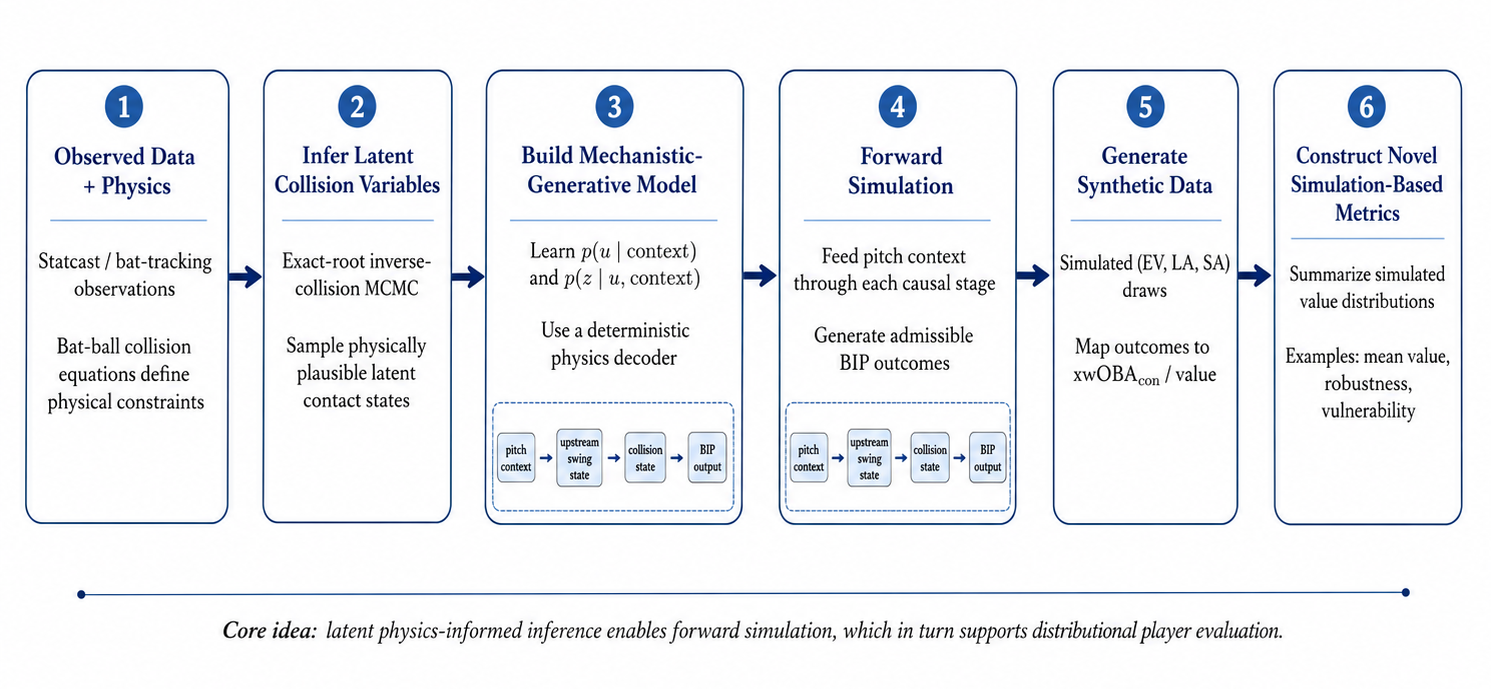
\includegraphics[
        width=0.82\textwidth,
        height=0.34\textheight,
        keepaspectratio
    ]{logical_flow_of_paper_process.png}
    \caption{Logical flow of the proposed BIP generative modeling framework: infer latent collision variables, train a mechanistic-generative simulator, generate synthetic BIP outcomes, and construct simulation-based player metrics.}
    \label{fig:logical_flow_paper}
\end{figure}

Constraining a generative or predictive machine learning model to learn within the limits of physical plausibility is a worthwhile addition by itself. However, for complex systems where building models or inference engines over high-dimensions creates computational and run-time issues, adding structural constraints limits the dimensionality of the hypothesis space. In order to learn latent collision variables, we use physical constraints, which allows sampling from a lower dimensional manifold embedded within higher dimensional space. The use of reduced manifold sampling to a physics-constrained sports application is included in section four. \citep{karniadakis2021physicsinformed,willard2022integrating,deistler2025simulation}. 

We believe that the ability to model the data-generating process of the collision system gives way to a fascinating new avenue in baseball intelligence. Specifically, for simulation of hypothetical in-game situations and the ability to ask counterfactual questions regarding pitch locations, bat speeds, and pitch speeds among others. We show intervention and synthetic data generation capabilities gives way to the idea of \textit{Generative Sabermetrics}. We put forward a subclass of Generative Sabermetrics, Robustness Metrics, which  analyzes hitter performance variance against all possible pitch types. This is a very difficult question to approach with empirical data alone due to the fact that most hitters don't have sufficient samples against every pitch type. However, replication of the data-generating process allows us to overcome empirical sparsity and expand the class of questions we are able to ask about the game of baseball \citep{le2017datadrivenghosting,carpenterBaseballSimulation}.




In the second section, we give an overview of the collision process within the collision system. In the third section, we define the collision system theoretically as a complex, dynamical system. In the fourth section, we use physical constraints of the collision process to augment our dataset to include latent collision variables via direct manifold sampling. In the fifth section, we design Mixture Density Network's (MDN), a generative modeling architecture, to represent the transition kernels (hitter tendencies) within the collision process. In the sixth section, we show our mechanistic generative model can directionally reproduce previous works within baseball analytics. Lastly, we extend our modeling framework to a new application: \textit{Generative Sabermetrics}. 


\section{Physics of the Bat-Ball Collision: The Data Generating Process}

In early literature, the ball-bat collision was viewed under rigid-body mechanics and only in the normal direction. This means that the bat was assumed to be non-flexible and have constant characteristics across the barrel. These assumptions are analytically tractable, but the bat-ball collision was later shown to be more comprehensively modeled in a dynamic, flexible manner with the bat having the ability to vibrate and bend during contact. A useful reduced form of the modern state of the bat-ball collision understanding is as a dynamic, flexible model where the bat-ball collision can be decomposed into two lossy springs: One spring representing energy transfer in the normal direction and one spring representing energy transfer in the tangential direction. \citep{nathan2000dynamics,cross1999impact,cross2006scattering,kensrud2017oblique, nathan2003characterizing}

An important distinction is the difference between the tangential and the normal directions. Intuitively, the normal direction refers to the direction created by extending a vector from the center of the barrel of the bat through the center of the pitch as the two objects collide. 

Formally, let \(c_{\mathrm{bat}}\in\mathbb{R}^3\) \footnote{The three dimensions are the x, y, and z dimensions of physical space} denote the center of the bat barrel at the point of contact, and let \(c_{\mathrm{ball}}\in\mathbb{R}^3\) denote the center of the baseball at impact. The unit normal direction is defined as
\[
\hat{\mathbf{n}}
=
\frac{c_{\mathrm{ball}}-c_{\mathrm{bat}}}
{\left\|c_{\mathrm{ball}}-c_{\mathrm{bat}}\right\|}.
\]
The tangential direction refers to the direction which is perpendicular to the normal direction. Formally, the tangential directions are all vectors lying in the plane orthogonal to \(\hat{\mathbf{n}}\), defined as
\[
\mathcal{T}_{\hat{\mathbf{n}}}
=
\left\{
\mathbf{v}\in\mathbb{R}^3:
\mathbf{v}\cdot \hat{\mathbf{n}}=0
\right\}.
\]
A unit tangential direction \(\hat{\mathbf{t}}\) is therefore any vector satisfying
\[
\hat{\mathbf{t}}\in \mathcal{T}_{\hat{\mathbf{n}}},
\qquad
\|\hat{\mathbf{t}}\|=1,
\qquad
\hat{\mathbf{t}}\cdot \hat{\mathbf{n}}=0.
\] Our physical world exists in 3-dimensional space, and thus the possibilities of where the tangential vector can fall holding the normal vector constant is a 2-dimensional plane. This distinction will become relevant in the following section when we make assumptions to reduce dimensionality for inference.

\begin{figure}[H]
    \centering
    \includegraphics[
        width=0.85\textwidth,
        height=0.42\textheight,
        keepaspectratio
    ]{normal_tangential_visual.png}
    \caption{\footnotesize Normal and tangential directions at the bat--ball contact point.}
    \label{fig:normal_tangential_visual}
\end{figure}

We define the collision process as the data-generating process from the pitch being released to the ball being put in play by the hitter. This collision process takes place within the collision system which we will define in more detail in the next section. The collision process is defined in three discrete time indexed stages: Pre-collision stage, collision stage, and post-collision stage. 

In the pre-collision stage, the pitch travels in the direction of the hitter with an initial velocity, decomposed into normal and tangential initial velocity, and spin. The hitter also has bat speed in the normal and tangential directions. The normal and tangential directions are not realized until collision, however it is useful conceptually and mathematically to decompose pre-collision velocities into the tangential and normal components.

During the collision stage, the bat makes contact with the pitch at some point along the barrel of the bat, denoted by x, at an angle, denoted \(\psi\), which measures the orientation of the baseball's center relative to the local bat-barrel contact frame at impact. Energy is then transferred from the bat to the ball and vice versa. The extent of the energy transferred to the ball versus transformed into other forms of energy is parametrized by the normal coefficient of restitution, \(e_y\), and the tangential coefficient of restitution, \(e_x\).\citep{nathan2003characterizing,cross1999impact,kensrud2017oblique}

For the post-collision stage, the ball exits with some exit velocity (EV), launch angle (LA), and spray angle (SA).\footnote{Exit velocity is the speed of the baseball immediately after contact with the bat, typically measured in miles per hour. Launch angle is the vertical angle at which the baseball leaves the bat, measured relative to the horizontal plane. Spray angle is the horizontal direction of the batted ball relative to the field of play, describing whether the ball is hit toward the pull side, center field, or the opposite field.}

\begin{figure}[H]
    \centering
    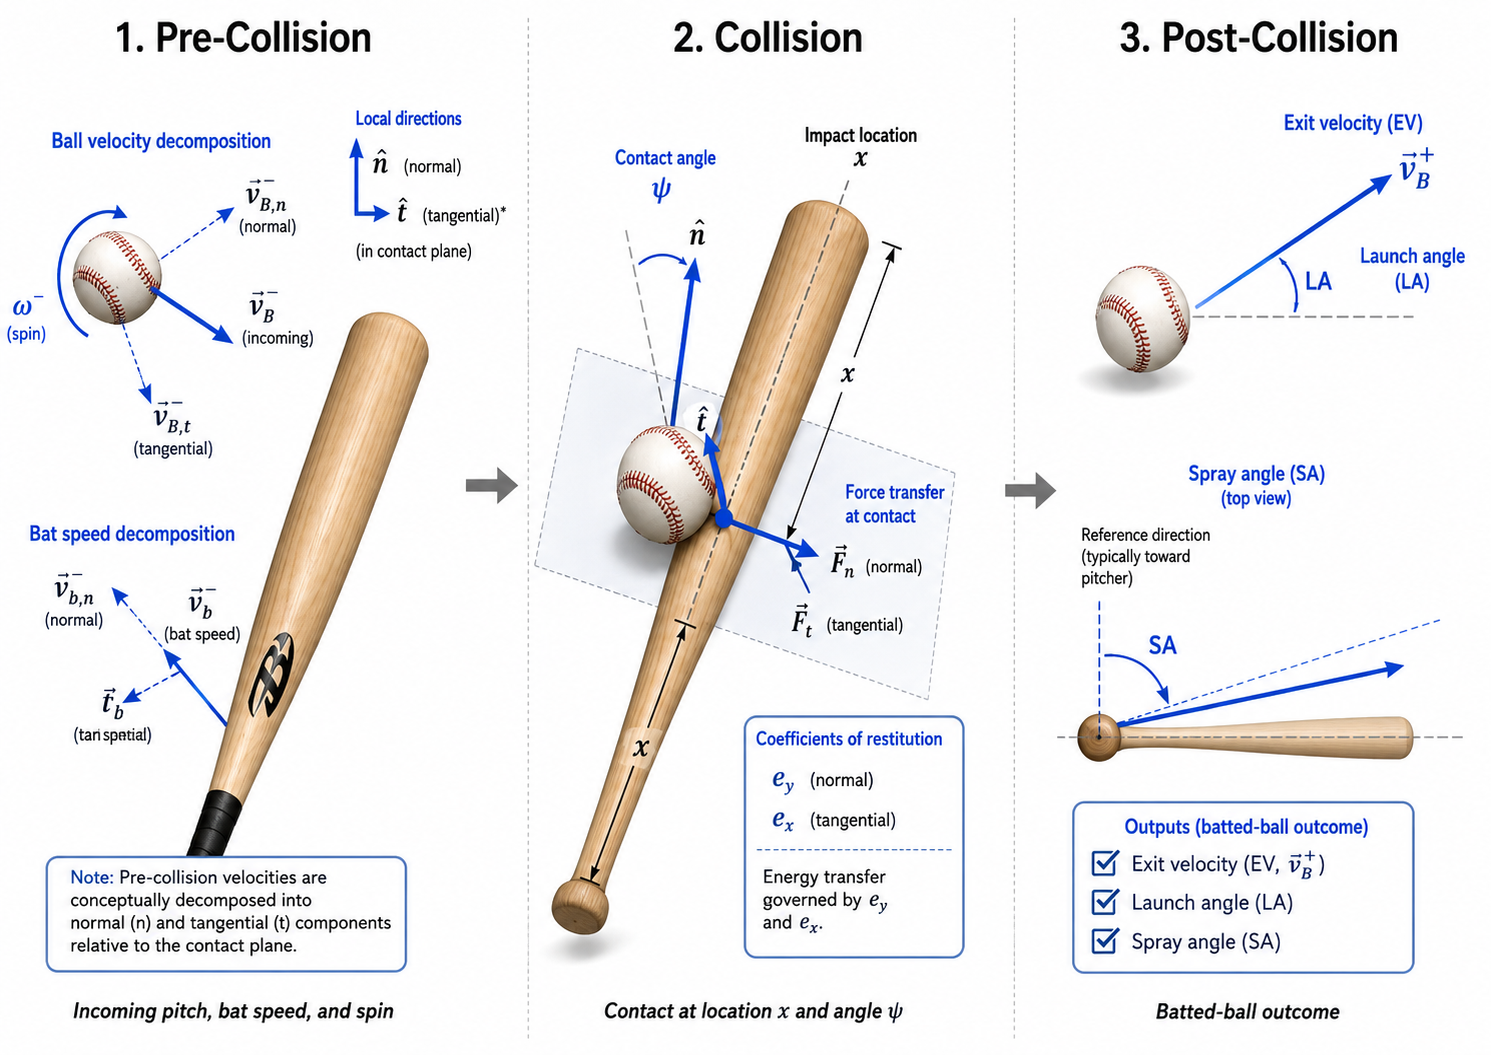
\includegraphics[
        width=0.95\textwidth,
        height=0.55\textheight,
        keepaspectratio
    ]{collision_stages.png}
    \caption{\footnotesize Three stages of the bat--ball collision: pre-collision decomposition, contact-stage force transfer, and post-collision batted-ball outcome.}
    \label{fig:collision_stages}
\end{figure}

The collision stage is where the interesting physics occurs. The ball and bat interact in two directions, as defined above. The normal impulse accounts for much of the force transfer and exit-speed generation. As the ball compresses, it stores kinetic energy as elastic potential energy, and then expands. However, most of the energy is dissipated as heat and internal deformation loss \citep{nathan2000dynamics,nathan2003characterizing}. More specifically, the kinetic energy after separation is split among:

\begin{itemize}
    \item Outgoing kinetic energy of the baseball
    \item Rigid-body rotation of the bat
    \item Vibrational energy in the bat
    \item Energy lost in compression and expansion of the ball
\end{itemize}

The coefficients of restitution dictate how energy is lost and transferred in each direction. The normal direction is primarily dictated by where the ball hits on the bat relative to the knob, sweet spot, and cap of the bat. The tangential direction is primarily dictated by the obliquity of the contact or the extent of the “glancing of contact”. \citep{cross1999impact,cross2006scattering,kensrud2017oblique,nathan2012spin}

The bat--ball collision was first characterized by a rigid-body collision model which described contact purely in the normal direction \citep{nathan2000dynamics,nathan2003characterizing}:

\begin{equation}
v_{B,n}^{+}
=
v_{B,n}^{-}
+
\frac{1+e_y}{1+r_y}
\left(
v_{b,n}^{-}-v_{B,n}^{-}
\right),
\label{eq:normal_velocity}
\end{equation}

where $v_{B,n}^{+}$ is the post-collision normal velocity of the baseball, $v_{B,n}^{-}$ is the pre-collision normal velocity of the baseball, $v_{b,n}^{-}$ is the pre-collision normal velocity of the bat at the contact point, $e_y$ is the normal coefficient of restitution, and $r_y$ is the effective normal recoil factor of the bat--ball system.

However, \citet{cross2006scattering} found that understanding the normal direction, while the primary driver of most contact events, is not complete in determining batted ball characteristics. The tangential component primarily represents the frictional interaction between the bat and the pitch and effects outgoing spin of the ball with some effect on the exit velocity. \citet{kensrud2017oblique} The tangential-compliance framework describes three distinct tangential regimes, where each one corresponds to a distinct batted-ball behavior: stick-slip, slip-stick-slip, and gross slip. Each tangential regime corresponds to a distinct effect which frictional forces have on the contact event. 

The outgoing velocity component in the tangential direction is:

\begin{equation}
v_{B,t}^{+}
=
v_{B,t}^{-}
+
\frac{\alpha(1+e_x)}
{(1+r_x)(1+\alpha)}
\left(
v_{b,t}^{-}
-
v_{B,t}^{-}
-
r\omega^{-}
\right),
\label{eq:tangential_velocity}
\end{equation}

where $v_{B,t}^{+}$ is the post-collision tangential velocity of the baseball, $v_{B,t}^{-}$ is the pre-collision tangential velocity of the baseball, $v_{b,t}^{-}$ is the pre-collision tangential velocity of the bat at the contact point, $e_x$ is the tangential coefficient of restitution, $r_x$ is the effective tangential recoil factor, $\alpha$ is the baseball inertia parameter, $r$ is the baseball radius, and $\omega^{-}$ is the pre-collision spin component relevant to tangential contact. For future reference, define $\omega^{+}$ as the post-collision spin component of the baseball. 

A full definition set of the variables related to the data generating process of the bat-ball collision can be found in the appendix.

The PyBaseball Statcast dataset either includes or allows for approximation of all pre-collision and post-collision variables that parametrize the bat-ball collision constraints which explain the collision process. However, the collision variables
\[
z
=
\left(
x,\ e_y^{\ast},\ \psi,\ e_x,\ \omega^{+}
\right)
\]
are not included in the PyBaseball Statcast dataset. Thus in order to model the collision process wholly, we must augment our dataset to include these latent collision variables. In the next section, we perform event-level inference of the latent-collision variables which are constrained by the physics of the bat-ball collision.

\section{Inverse Latent Collision Variable Inference}

Under a few assumptions, a Metropolis-Hastings Markov Markov Chain Monte Carlo (MH MCMC) algorithm can be constructed which incorporates the bat-ball collision constraints of Kelsrud and Nathan, to sample latent collision variables for BIP events where pre and post collision variables are observed. These bat-ball collision constraints are integrated into the sampling methodology creating a physically plausible latent collision variable manifold. The MH MCMC algorithm samples directly from this manifold, enforcing physical admissibility, and then weights each sample by priors constructed via previous studies and experimentation. Making use of the constraints which bound the bat-ball collision via direct manifold sampling allows for effective dimensionality reduction of the posterior and sampling distributions.

\begin{figure}[H]
    \centering
    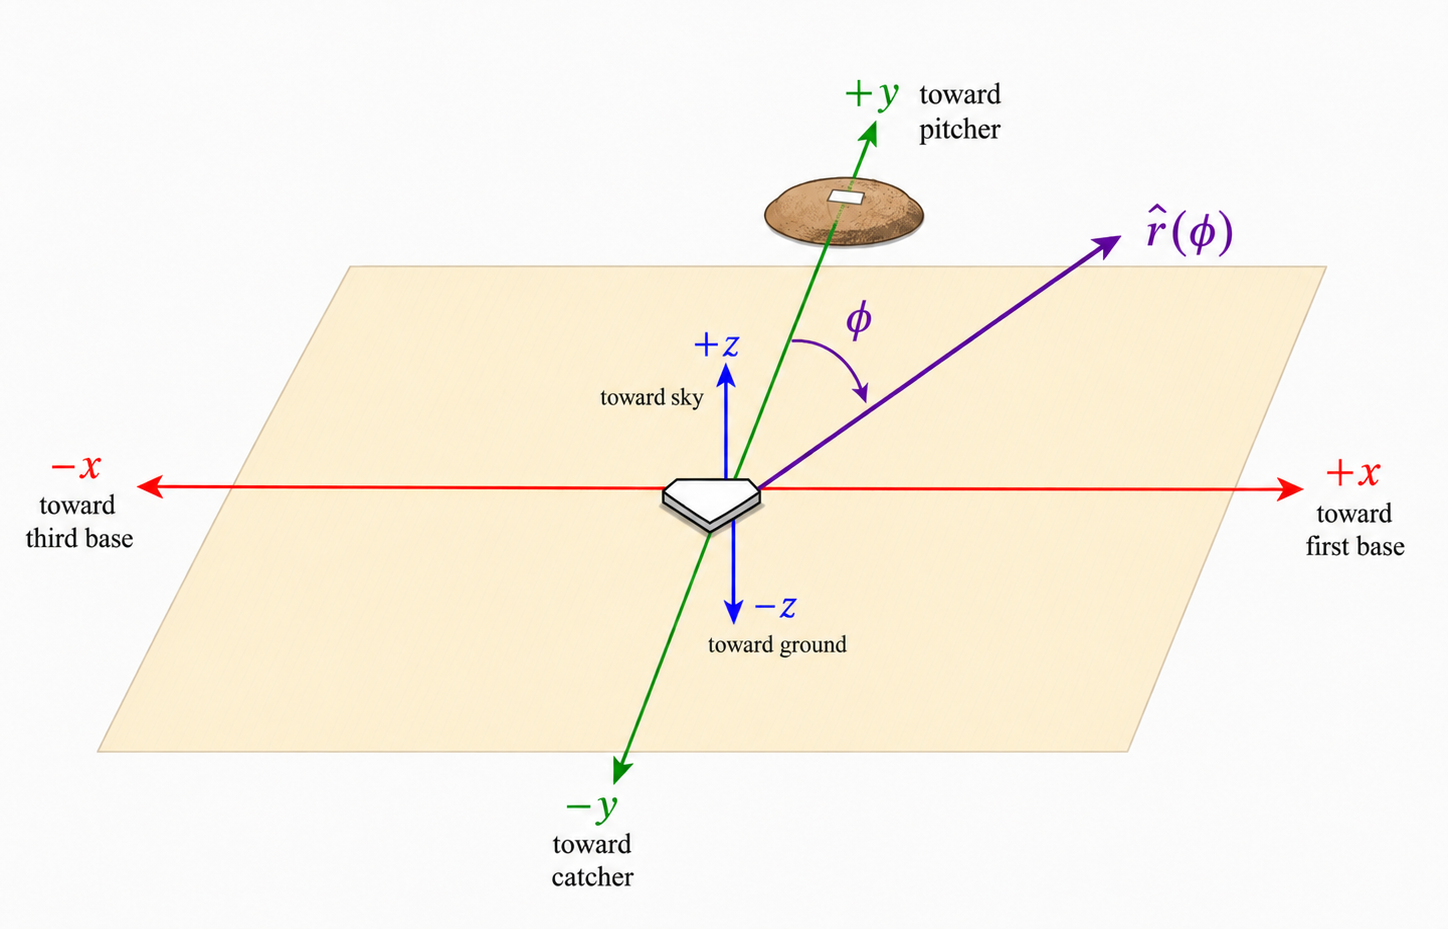
\includegraphics[width=0.85\textwidth]{coordinate_basis.png}
    \caption{Global coordinate system in the home plate frame.}
    \label{fig:coordinate-basis}
\end{figure}


\subsection{Coplanar Re-Parametrization Assumption}

We made the assumption that the collision event is coplanar. We observe the outgoing batted ball direction up until measurement noise. Thus, we are able to reconstruct the outgoing directional vector from the data. However, we do not observe the tangential or normal directions that compose the outgoing batted ball direction. The coplanar assumption is that the normal and tangential vectors lie within the plane spanned by the z-unit vector and the outgoing batted ball unit vector. Under this assumption, the model enforces zero out-of-plane impulse and therefore rules out side-spin components that would produce lateral deviation out of the scattering plane. 

The ideology of the coplanar re-parametrization is as follows:

Define the radial direction as
\begin{equation}
\hat{r}(\phi) = \sin \phi \hat{\mathbf{x}} + \cos \phi \hat{\mathbf{y}} ,
\tag{4}
\end{equation}

Define the horizontal direction orthogonal to spray direction by
\begin{equation}
\hat{c}(\phi) = \hat{r}(\phi) \times \hat{\mathbf{z}}
= \cos \phi \hat{\mathbf{x}} - \sin \phi  \hat{\mathbf{y}} .
\tag{5}
\end{equation}

where \(\phi\) is the spray angle which we derived from the Statcast PyBaseball dataset using the methodlologies of \citep{petti2017statcastexport}.

\(\hat{\mathbf{x}}\) is the basis vector of the x-direction, where the positive x-direction points toward first base and the negative x-direction points toward third base.

\(\hat{\mathbf{y}}\) is the basis vector of the y-direction, where the positive y-direction points toward the pitcher and the negative y-direction points toward the catcher.

\(\hat{\mathbf{z}}\) is the basis vector of the z-direction, where the positive z-direction points toward the sky and the negative z-direction points toward the ground.

We assume the origin for this vector space is at home plate. Refer to figure 4. 

Under the coplanar assumption, the scattering plane is

\begin{equation}
\Pi(\phi) = \operatorname{span}\left[\hat{r}(\phi), \hat{\mathbf{z}}\right].
\tag{6}
\end{equation}



Parameterize the collision normal by

\begin{equation}
\hat{n}(\psi, \phi) = \cos \psi \hat{r}(\phi) + \sin \psi \hat{\mathbf{z}} ,
\tag{7}
\end{equation}

Where \(\psi\) is measured as the angle between the normal direction and the radial direction

Define the in-plane tangential direction by

\begin{equation}
\hat{t}(\psi, \phi) = - \sin \psi \hat{r}(\phi) + \cos \psi \hat{\mathbf{z}} .
\tag{8}
\end{equation}

Conditional on the observed launch angle \(\theta\), and spray angle, \(\phi\), the decomposition of the outgoing velocity into the normal-tangential frame depends only on the latent collision angle \(\psi\).

Additionally, the observed outgoing unit direction is

\begin{equation}
\hat{v}_{obs} = \cos \theta \hat{r}(\phi) + \sin \theta \hat{\mathbf{z}}
  \tag{9}
  \end{equation}

The computational benefits of this assumption are two fold:

1.) We are able to parametrize the normal and tangential vectors with a single unknown parameter, \(\psi\), instead of two. This reduces the dimensionality of inference over the latent collision variables.

2.) The observed spray angle fixes the plane perpendicular to the scattering plane. If the bat is locally approximated as a cylinder whose cross-sectional collision dynamics occur in this plane, then the bat-axis direction is determined up to sign by the cross-plane direction $\hat{c}(\phi)$

More experimentation is needed to find if this assumption is robust. However, for the purposes of our framework and study we will assume it is.

\subsection{Derivation of Bat-Ball Collision Constraints}

For the following equations, if a variable is given in functional form, this denotes that the variable is either a deterministic or stochastic function of the variable which parametrizes it. While more variables may be necessary to represent the actual value of the given variable, we only denote the latent collision variables that comprise a given variable used in the given bat-ball collision constraint. An exhaustive list of variable definitions are listed in the appendix, however for this section the focus is on deriving the three constraining equations which allow for physically plausible or manifold constrained sampling of the latent collision variables. Thus, much of the physical meaning is glossed over, opting for mathematical derivations. The collision equations below adapt the normal and oblique bat--ball collision formalisms developed in the baseball physics literature \citep{nathan2000dynamics,nathan2003characterizing,cross2006scattering,kensrud2017oblique}.

We now derive normal, tangential, and spin constraints. When when used in coordination with the previous coplanar assumption will reduce a 4-dimensional inverse inference problem to a 1-dimensional inverse inference problem.

For a proposed contact location x, define the offset from the bat center of mass

\begin{equation}
b(x) = x - x_{cm},
\tag{14}
\end{equation}

along with the normal and tangential recoil factors

\begin{equation}
r_y(x)
=
m
\left(
\frac{1}{M} + \frac{b(x)^2}{I_0}
\right),
\quad
r_x(x)
=
\frac{m\alpha}{1+\alpha}
\left(
\frac{1}{M} + \frac{b(x)^2}{I_0} + \frac{R^2}{I_z}
\right).
\tag{15}
\end{equation}

Then the normal collision equation, reintroduced, is

\begin{equation}
v_{B,n}^+
=
v_{B,n}^-
+
\frac{1 + e_y(x)}{1 + r_y(x)}
\left(
v_{b,n}^- - v_{B,n}^-
\right).
\tag{17}
\end{equation}

where \(e_y(x)\) is assumed to be drawn from a distribution parameterized by \(x\). This is supported by \cite{nathan2000dynamics}.

Substituting \(v_{B,n}^+ = s \cos(\theta - \psi)\) gives the normal constraint

\begin{equation}
F_n(x, \psi; m_{obs})
=
v_{B,n}^-(\psi)
+
\frac{1 + e_y(x)}{1 + r_y(x)}
\Delta_n(\psi)
-
s \cos(\theta - \psi)
=
0.
\tag{18}
\end{equation}

Where s is the observed exit velocity.

The tangential collision equation, reintroduced, is

\begin{equation}
v_{B,t}^+
=
v_{B,t}^-
+
\frac{\alpha(1+e_x)}
{(1+r_x(x))(1+\alpha)}
\left(
v_{b,t}^- - v_{B,t}^- - r\omega^-
\right).
\tag{19}
\end{equation}

Substituting \(v_{B,t}^+ = s \sin(\theta - \psi)\) gives the tangential constraint

\begin{equation}
F_t(x, e_x, \psi; m_{obs})
=
v_{B,t}^-(\psi)
+
\frac{\alpha(1+e_x)}
{(1+r_x(x))(1+\alpha)}
\Delta_t(\psi)
-
r\omega^-
-
s\sin(\theta-\psi)
=
0.
\tag{20}
\end{equation}

where \(\alpha\) and \(r\) are exogenous parameters assumed to be constant.

Whenever the denominator is nonzero, this yields the implied tangential restitution

\begin{equation}
e_x(x, \psi)
=
\frac{(1+r_x(x))(1+\alpha)}
{\alpha\Delta_t(\psi,\phi)-r\omega^-}
\left[
s\sin(\theta-\psi)-v_{B,t}^-(\psi,\phi)
\right]
-
1.
\tag{21}
\end{equation}

The spin update constraint is

\begin{equation}
\alpha r(\omega^+ - \omega^-)
=
v_{B,t}^- - v_{B,t}^+
-
\frac{D}{r}v_{B,n}^+.
\tag{22}
\end{equation}

Substituting the exact observed-speed components gives the spin constraint

\begin{equation}
F_\omega(x, \psi, \omega^+; m_{obs})
=
\alpha r(\omega^+-\omega^-)
-
v_{B,t}^-(\psi,\phi)
-
s\sin(\theta-\psi)
+
\frac{D}{r}s\cos(\theta-\psi)
=
0,
\tag{23}
\end{equation}

and therefore

\begin{equation}
\omega^+(x,\psi)
=
\omega^-
+
\frac{
v_{B,t}^-(\psi,\phi)
-
s\sin(\theta-\psi)
-
Ds\cos(\theta-\psi)/r
}
{\alpha r}.
\tag{24}
\end{equation}

Thus, once directionality, spin, and velocities are enforced to be consistent with the constraints that dictate the bat-ball collision, each event becomes fully identified up to root variable sampling. The proof is given by the implicit function theorem in the next section.

\subsection{Physically Plausible Manifold Embedding in Latent Collision Variable Space}

The inverse-collision problem can be thought of as a search for physically plausible values of the 
four-dimensional latent collision state
\[
\ell
=
(x,\psi,e_x,\omega^{+})
\in \mathbb{R}^4,
\]
where $x$ is the location of the impact, $\psi$ is the contact angle, $e_x$ is the tangential 
coefficient of restitution, and $\omega^{+}$ is the spin component after collision. 

Without physical constraints from previous experimentation, inference over $\ell$ would require searching over an
unconstrained four-dimensional latent space. However, the bat--ball collision
equations impose three equality constraints:
\[
F_n(x,\psi;m^{\ast},e_y^{\ast}) = 0,
\]
\[
F_t(x,\psi,e_x;m^{\ast},e_y^{\ast}) = 0,
\]
\[
F_{\omega}(x,\psi,\omega^{+};m^{\ast},e_y^{\ast}) = 0.
\]
Equivalently, the constraint map is defined as
\[
F:
\mathbb{R}^4
\rightarrow
\mathbb{R}^3,
\qquad
F(\ell)
=
\begin{pmatrix}
F_n(x,\psi;m^{\ast},e_y^{\ast}) \\
F_t(x,\psi,e_x;m^{\ast},e_y^{\ast}) \\
F_{\omega}(x,\psi,\omega^{+};m^{\ast},e_y^{\ast})
\end{pmatrix}.
\]


Let \(m^{\ast}\) denote all plausible observation measurements within sensor error, and let \(e_y^{\ast}\) denote all plausible values of \(e_y\) given x. Conditional on these quantities, the physically feasible exact-collision set is defined as
\[
\mathcal{M}_0(m^{\ast}, e_y^{\ast})
=
\left\{
(x,\psi,e_x,\omega^{+}) \in \mathbb{R}^4
:
F(x,\psi,e_x,\omega^{+}) = 0,
\ A(x,\psi,e_x,\omega^{+};m^{\ast}) = 1
\right\},
\]
where $A(\cdot)$ is an admissibility indicator enforcing the physically allowed
domain, including support restrictions, sign restrictions, nonsingular
denominators, tangential-regime validity, and finite prior density. Admissibility constraints and exact rationale are defined in greater detail in the following subsection.

The key dimensionality reduction follows from the Implicit Function Theorem.
Let
\[
J_{(\psi,e_x,\omega^{+})}F
=
\frac{\partial(F_n,F_t,F_{\omega})}
{\partial(\psi,e_x,\omega^{+})}
\]
denote the Jacobian of the constraint equations with respect to the three
variables $(\psi,e_x,\omega^{+})$. If, at an admissible solution
\[
(x_0,\psi_0,e_{x,0},\omega_0^{+}),
\]
this Jacobian has full rank,
\[
\det
\left[
J_{(\psi,e_x,\omega^{+})}F
\right]
\neq 0,
\]
then there exists a neighborhood of $x_0$ and continuously differentiable
functions
\[
\psi(x), \qquad e_{x}(x), \qquad \omega^{+}(x)
\]
such that all nearby admissible solutions can be written as
\[
\ell(x)
=
\left(
x,\psi(x),e_{x}(x),\omega^{+}(x)
\right).
\]

with
\begin{align}
\psi(x)
&=
\operatorname{atan2}\!\left(-A(x),B(x)\right),
\\[0.75em]
e_x(x)
&=
\frac{\left(1+r_x(x)\right)(1+\alpha)}
{\alpha\left(\Delta_t(\psi(x))-r\omega^{-}\right)}
\left[
s\sin\!\left(\theta-\psi(x)\right)
-
v^{-}_{B,t}(\psi(x))
\right]
-1,
\\[0.75em]
\omega^{+}(x)
&=
\omega^{-}
+
\frac{
v^{-}_{B,t}(\psi(x))
-
s\sin\!\left(\theta-\psi(x)\right)
-
\frac{D}{r}s\cos\!\left(\theta-\psi(x)\right)
}
{\alpha r}.
\end{align}

Locally, the four-dimensional latent collision solution set is a
one-dimensional manifold embedded in $\mathbb{R}^4$. The physical constraints
reduce the effective search problem from an unconstrained search over
$(x,\psi,e_x,\omega^{+})$ to a constrained search over the root coordinate $x$. This substantially reduces the
effective hypothesis space and prevents the sampler from assigning posterior
mass to latent states that may be statistically convenient but physically
impossible.

\subsection{Inverse Latent Collision Variable Sampling}

Due to observation measurement error and uncertain results regarding some physical variables in previous works, we utilize Bayesian methodologies to address the uncertainty surrounding relevant variables via priors.

Because the observed Statcast and bat-tracking variables are measured with sensor error, we do not treat the raw measurement block as exact. Instead, for each observed event we introduce a latent measurement block
\[
m^{\ast}
=
\Big(
s^{\ast},
\theta^{\ast},
h_{c,x}^{\ast},
h_{c,y}^{\ast},
v_b^{\ast},
a^{\ast},
d^{\ast},
v_{x0}^{\ast},
v_{y0}^{\ast},
v_{z0}^{\ast},
a_x^{\ast},
a_y^{\ast},
a_z^{\ast},
y_0^{\ast},
\omega_{\mathrm{spin}}^{\ast},
\gamma_{\mathrm{axis}}^{\ast}
\Big),
\]
where each component is centered at its observed value in
\[
m^{\mathrm{obs}}
=
\Big(
s^{\mathrm{obs}},
\theta^{\mathrm{obs}},
h_{c,x}^{\mathrm{obs}},
h_{c,y}^{\mathrm{obs}},
v_b^{\mathrm{obs}},
a^{\mathrm{obs}},
d^{\mathrm{obs}},
v_{x0}^{\mathrm{obs}},
v_{y0}^{\mathrm{obs}},
v_{z0}^{\mathrm{obs}},
a_x^{\mathrm{obs}},
a_y^{\mathrm{obs}},
a_z^{\mathrm{obs}},
y_0^{\mathrm{obs}},
\omega_{\mathrm{spin}}^{\mathrm{obs}},
\gamma_{\mathrm{axis}}^{\mathrm{obs}}
\Big).
\]

The inverse sampling architecture uses an independent Gaussian measurement-error model:
\[
p(m^{\ast}\mid m^{\mathrm{obs}})
=
\prod_{j}
\mathcal{N}
\left(
m_j^{\ast};
m_j^{\mathrm{obs}},
\sigma_j^2
\right),
\]

The sensor-error scales $\sigma_j$ are fixed numerical values in the production exact-root MCMC implementation. Refer to the appendix for the exact prior noise scales.

The preceding manifold argument shows that, for a fixed denoised measurement draw
$m^{\star}$ and sampled normal restitution parameter $e_y^{\star}$, the collision
constraints reduce the latent collision state from an unconstrained four-dimensional
search over
\[
(x,\psi,e_x,\omega^+)
\]
to a one-dimensional search over impact location $x$. The
inverse-collision sampler exploits this reduction directly. Rather than
sampling freely over $(x,\psi,e_x,\omega^+)$, the Markov chain proposes values of
\[
(x,m^{\star},e_y^{\star}),
\]
solves the exact-root normal equation for admissible contact-angles,
$\psi$, and then deterministically computes the implied tangential restitution
$e_x$ and post-collision spin $\omega^+$.

Thus, each proposed low-dimensional state induces a candidate augmented collision state
\[
(x,m^{\star},e_y^{\star})
\quad \longrightarrow \quad
\left(
x,m^{\star},e_y^{\star},\psi_j,e_{x,j},\omega_j^+
\right).
\]

A candidate branch is accepted as physically admissible only if all admissibility checks pass. These include:


\begin{itemize}
    \item existence of a valid exact root within the allowed support;
    \item positive outgoing normal velocity, \(V_n^+ > 0\);
    \item bounded tangential-to-normal outgoing velocity ratio,
    \[
    \left| \frac{V_t^+}{V_n^+} \right| < 1;
    \]
    \item positive incoming normal relative velocity, \(d_n > 0\);
    \item nonsingularity of the tangential denominator used to solve for \(e_x\);
    \item satisfaction of the contact-geometry bound for \(D\);
    \item exclusion of the gross-slip regime;
    \item admissible support and finite prior density for \(e_x\);
    \item finiteness of the full log target.
\end{itemize}

Let \(A(s_j)\) denote the indicator that all physical admissibility conditions are
satisfied:
\[
A(s_j)
=
\mathbf{1}
\left\{
s_j \ \text{passes all production admissibility checks}
\right\}.
\]
Only states satisfying \(A(s_j)=1\) are assigned nonzero posterior density.

For an admissible state, the target density is
\begin{equation}
\log \pi
\left(
x,m^{\star},e_y^{\star},\psi,e_x,\omega^+
\right)
=
\log p(x)
+
\log p(m^{\star}\mid m^{\mathrm{obs}})
+
\log p(e_y^{\star}\mid x)
+
\log p(e_x\mid \mathrm{regime}),
\label{eq:mcmc_log_target}
\end{equation}
with the exact-root equations and admissibility constraints enforced as hard
indicators. Equivalently,
\[
\pi(s)
\propto
p(x)\,
p(m^{\star}\mid m^{\mathrm{obs}})\,
p(e_y^{\star}\mid x)\,
p(e_x\mid \mathrm{regime})\,
A(s).
\]

The proposal distribution operates on the variables that are sampled directly:
\[
(x,m^{\star},e_y^{\star}).
\]
The production sampler uses a reflected random-walk proposal for \(x\) on the
barrel support interval,
\[
x \in [L-11,L],
\]
a Gaussian perturbation model for the denoised measurement block \(m^{\star}\),
and a truncated-normal proposal/prior structure for \(e_y^{\star}\). Therefore,
a proposal from the current state \(s^{(t)}\) can be written schematically as
\[
x' \sim q_x(x'\mid x^{(t)}),
\]
\[
m^{\star\prime} \sim q_m(m^{\star\prime}\mid m^{\star(t)}),
\]
\[
e_y^{\star\prime} \sim q_y(e_y^{\star\prime}\mid e_y^{\star(t)},x'),
\]


Let the proposed admissible augmented state be
\[
s'
=
\left(
x',
m^{\star\prime},
e_y^{\star\prime},
\psi',
e_x',
\omega^{+\prime}
\right),
\]
and let the current state be
\[
s^{(t)}
=
\left(
x^{(t)},
m^{\star(t)},
e_y^{\star(t)},
\psi^{(t)},
e_x^{(t)},
\omega^{+(t)}
\right).
\]
The Metropolis--Hastings log acceptance ratio is
\begin{equation}
\log \alpha
=
\left[
\log \pi(s')
-
\log \pi(s^{(t)})
\right]
+
\left[
\log q(s^{(t)}\mid s')
-
\log q(s'\mid s^{(t)})
\right].
\label{eq:mh_acceptance_ratio}
\end{equation}

The Markov chain transition is then
\[
s^{(t+1)}
=
\begin{cases}
s', & \text{with probability } \min\{1,\exp(\log \alpha)\}, \\[4pt]
s^{(t)}, & \text{otherwise}.
\end{cases}
\]

The resulting posterior draws are therefore samples from the physically
admissible exact-root manifold:
\[
s^{(k)}
=
\left(
x^{(k)},
m^{\star(k)},
e_y^{\star(k)},
\psi^{(k)},
e_x^{(k)},
\omega^{+(k)}
\right),
\qquad
k=1,\ldots,250.
\]
These draws provide event-specific posterior samples over latent collision states.
The crucial feature of the algorithm is that the sampler does not explore arbitrary
latent collision configurations. It proposes only the directly sampled variables,
solves the collision equations exactly, rejects inadmissible proposals, and therefore
samples directly from the manifold of physically-plausible collision explanations. This strategy is conceptually related to constrained or manifold MCMC methods, which exploit lower-dimensional structure induced by equality constraints \citep{brubaker2012family,byrne2013geodesic}.

We now have augmented the directly observed or approximated pre and post collision variables and exogenous assumed variables with probabilistically weighted physically plausible samples of the latent collision variables. We now have an augmented data set which acts as a noisy representation of many collision process realizations. We now outline a theoretical proposal of the collision system as a complex dynamical system before employing generative architectures to model the transition kernels of the collision system.

\section{The Collision System: A Complex Dynamical System}

We start with a few critical definitions:

Von Bertalanffy defined a system as elements standing in interrelation among themselves and with the environment (Bertalanffy, 1968).

A complex system is a system composed of many interacting components whose collective behavior is not trivially reducible to, or predictable from, the behavior of the individual components alone \cite{newman2011complex}. 

A dynamical system is a system who's state evolves over time according to an evolution rule, often producing nonlinear, emergent, or path-dependent behavior. A dynamical system is constrained to a given state-space which is defined as the set of all possible states of a dynamical system \cite{terman2008state}. 

A complex, dynamical system is one which fits all three of the prior definitions: A system composed of many interacting elements which interact which each other and the environments whose collective state evolves over time according to deterministic or stochastic rules.

We assume pitcher behavior \footnote{Pitcher behavior includes pitch selection, pitch location, etc.} can only be understood in the context of the game context, opposing hitter, etc. Likewise, we assume hitter behavior \footnote{Swing produced and subsequent BIP realization} can only be understood in the context of the opposing pitcher, pitch realization, game context, etc. Thus the criteria for a complex system is met.

The collision system fits the definition of a dynamical system as the evolution of the bat and the ball during the realization of a single pitch follow a spatiotemporal path during the pre-collision, collision, and post-collision stages. 

Thus, we outlay a model of the collision system as a discrete-time, continuous valued state space, complex, dynamical system.

\subsection{System State and Pitch-Level Generative Process}

Let (i) index a single pitch event. The state of the collision system for pitch (i) is represented by the staged vector
\begin{equation}
s_i = (c_i,u_i,z_i,e_i),
\end{equation}
where each component corresponds to a distinct stage of the collision process. The pre-collision pitch state is denoted by
\begin{equation}
c_i \in \mathcal{C},
\end{equation}
and contains the pitch and game-context variables available prior to contact. These may include pitch type, pitch velocity, pitch movement, pitch location, count, handedness, hitter identity, pitcher identity, and other observable contextual information.

The pre-collision swing state is denoted by
\begin{equation}
u_i \in \mathcal{U},
\end{equation}
and represents hitter-generated variables that describe the batter's response to the pitch before contact. These may include bat speed, swing plane, attack angle, timing, and related swing quantities.

The collision state is denoted by
\begin{equation}
z_i \in \mathcal{Z},
\end{equation}
and contains the physically meaningful variables that govern the bat-ball collision. These may include impact location, contact angle, coefficients of restitution, post-collision spin, and other latent variables required to characterize the collision geometry and impulse transfer.

The post-collision exit-outcome state is denoted by
\begin{equation}
e_i \in \mathcal{E},
\end{equation}
and contains the observed or modeled outcome variables generated after contact. These may include exit velocity, launch angle, spray angle, batted-ball value, or other outcome measures derived from the collision.

The full state is not observed simultaneously. Instead, it is revealed through a spatiotemporal process:
\begin{equation}
S_{i,0}
\longrightarrow
S_{i,1}
\longrightarrow
S_{i,2}
\longrightarrow
S_{i,3}.
\end{equation}
The staged states are defined as
\begin{align}
S_{i,0} &= c_i, \\
S_{i,1} &= (c_i,u_i), \\
S_{i,2} &= (c_i,u_i,z_i), \\
S_{i,3} &= (c_i,u_i,z_i,e_i).
\end{align}


Thus, \(S_{i,0}\) represents the initial pre-collision pitch state, \(S_{i,1}\) represents the state after the pre-collision swing variables have been generated, \(S_{i,2}\) represents the state after the latent collision variables have been generated, and \(S_{i,3}\) represents the terminal pitch-level state after the exit outcome has been generated.

\subsection{Transition Kernels}

The pitch-level generative process is decomposed into three conditional transition kernels. The pre-collision kernel generates the swing state conditional on the pitch context:
\begin{equation}
u_i \sim p_{\theta_U}(u_i \mid c_i).
\end{equation}
The collision kernel generates the latent collision state conditional on the pre-collision pitch state and the pre-collision swing state:
\begin{equation}
z_i \sim p_{\theta_Z}(z_i \mid u_i,c_i).
\end{equation}
The post-collision kernel generates the BIP realization state conditional on the pitch, swing, and collision states:
\begin{equation}
e_i \sim p_{\theta_E}(e_i \mid z_i,u_i,c_i).
\end{equation}

Together, these kernels define the staged generative sequence
\begin{equation}
c_i
\longrightarrow
u_i
\longrightarrow
z_i
\longrightarrow
e_i.
\end{equation}
Equivalently, the full pitch-level generative process is the composition of the three conditional kernels:
\begin{equation}
\begin{aligned}
p_{\theta}(e_i,z_i,u_i \mid c_i)
&=
p_{\theta_E}(e_i \mid z_i,u_i,c_i)
p_{\theta_Z}(z_i \mid u_i,c_i)
p_{\theta_U}(u_i \mid c_i).
\end{aligned}
\end{equation}

This factorization encodes the assumption that the BIP realization is generated through a structured sequence of stages. First, the swing state is generated from the observed pitch context. Second, the latent collision state is generated from the pitch context and swing state. Third, the BIP realization is generated from the combined pitch, swing, and collision states.

The conditional distribution of BIP realizations given the pitch context is obtained by marginalizing over the intermediate swing and collision states:
\begin{equation}
\begin{aligned}
p_{\theta}(e_i \mid c_i)
=
\int_{\mathcal{U}}
\int_{\mathcal{Z}}
&p_{\theta_E}(e_i \mid z_i,u_i,c_i)
p_{\theta_Z}(z_i \mid u_i,c_i) 
p_{\theta_U}(u_i \mid c_i)
dz_i du_i.
\end{aligned}
\end{equation}

Under this notation, the collision system defines the broader state space, structural or mechanistic relationships among the relevant variables, and temporal orderings of the state updates. A pitch which is put in play is one stochastic realization, or trajectory, through that system.



\section{Generative Collision Model}

We now extend the theoretical definition of the collision system as a complex, dynamical system to an applied context where we design and train models for each of the kernels in the collision process. 

We train Mixture Density Networks for the pre-collision and collision kernels. We then use a physics decoder to map the realized pitch, swing, and collision variables to a BIP realization. We use the augmented PyBaseball Statcast data set to train, calibrate, and test the MDNs. The output is that we are now able to simulate the swing and BIP realization for a given pitch type and location using the aforementioned model network.


\subsection{Model Assumptions}

We define a single realization of a pitch which is put in play within the collision system as following the collision process. For our model of the collision process, we make the assumption that the pitch context is supplied to the model or drawn from an initial distribution and that the hitter will make contact with the ball in fair play. This is a fair assumption to make, where this mechanistic generative model is assumed to be a component of a broader simulation where pitch context and swing decision are modeled separately by a model such as the LLM generative model of Ahn et. al. Our model specifically captures the continuous valued state space components, where physical structure is critical to the process.

We now map the states used in the training of the generative model onto the structure defined by the theoretical modeling of the collision system: 

 \textbf{Stage 0: Pre-Collision Swing State} The first step in the mechanistic pitcher-hitter process is the pitcher chooses a pitch and executes it. The pitch context gives all of the relevant metrics of the realized pitch including pitch speed, pitch spin, pitch location, etc.

Let the observed pitch context be:

\[
c = (g,p)
\]

Where

\begin{itemize}
    \item g: plate appearance and pitch context available at prediction time, such as count, plate location, pitch type, release speed, release spin rate, handedness, and related descriptors.
    \item p: fixed batter and bat quantities such as bat length, bat weight, center of mass, radius of gyration, and derived inertias.
\end{itemize}

\textbf{Stage 1: Pre-Collision Swing State} 
The second step in the pitcher-hitter process is that the batter executes a swing where swing metrics including bat speed, attack angle, and attack direction are realized. Given our coplanar reparameterization assumption, the attack direction and spray angle coincide. 

\[
u = (\tilde{v}_{ss}, \tilde{a}, \tilde{d}),
\]

\textbf{Stage 2: Collision Stage}
After the pitch is thrown and the hitter swings, the next step is for the bat to make contact with the ball. The collision variables are realized at this stage.

\[
z = (x, \psi, e_y^\star, e_x^\star, w^+),
\]

\textbf{Stage 3: Post-Collision BIP Realization}
The pitch context, upstream swing variables, and collision variables are then mapped to a BIP realization via a physics decoder.

BIP realizations are characterized by the (EV, LA, SA) triple.

\begin{figure}[H]
    \centering
    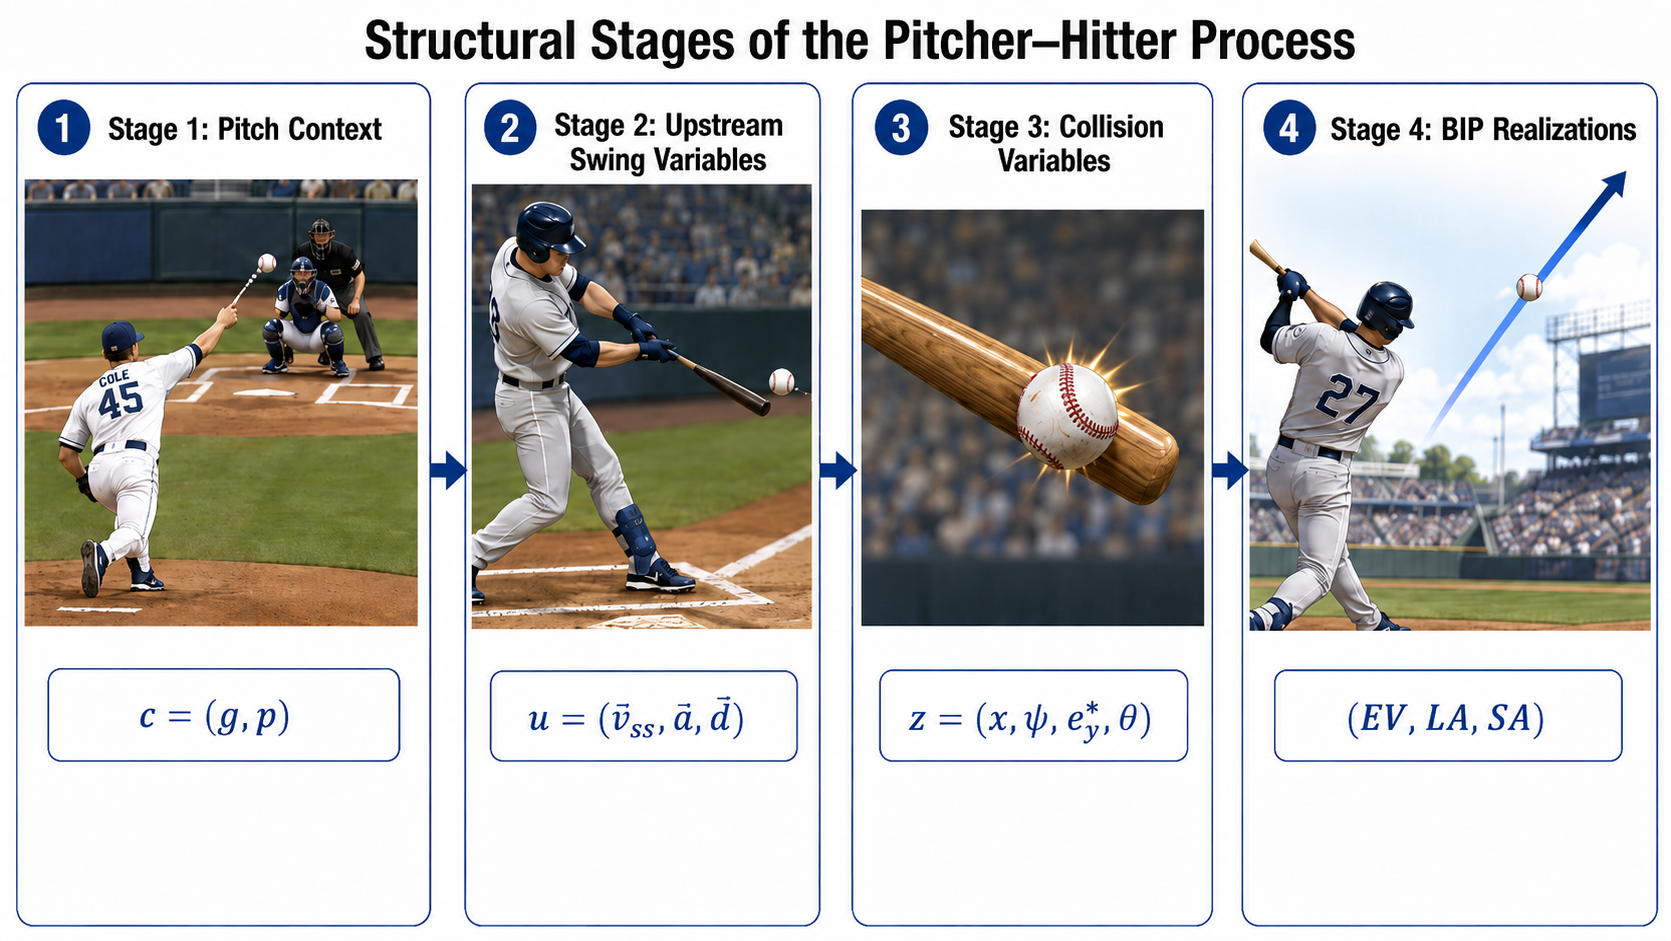
\includegraphics[width=\textwidth]{pitcher_hitter_process.png}
    \caption{Structural stages of the pitcher-hitter data generating process. The process begins with the realized pitch context, proceeds through upstream swing variables, then collision variables, and finally maps these inputs through a physics decoder to a batted-ball-in-play realization characterized by exit velocity, launch angle, and spray angle.}
    \label{fig:pitcher-hitter-process}
\end{figure}



The goal of the generative model pipeline is for a distribution over BIP realizations given the pitch context.

\[
P(EV, LA, SA | c)
\]

The complete factorization is therefore

\begin{equation}
P(EV, LA, SA | c)
=
\int
P(EV, LA, SA | u, z, c)
p_\phi(z | u, c)
p_\theta(u | c)
\,du\,dz,
\end{equation}

where the conditional distribution

\[
P(EV, LA, SA | u, z, c)
\]

is induced by a deterministic physics decoder plus hard admissibility filtering.




\subsection{Swing State Neural Density Estimator}

The upstream state is

\[
u = (\tilde{v}_{ss}, \tilde{a}, \tilde{d}).
\]


The stage-u model is a Mixture Density Network (MDN). More specifically a mixture Gaussian–von Mises network. Conditional on context, it produces mixture weights \(\pi_k(c)\) and, for each mixture component,

\begin{itemize}
    \item a full \(2 \times 2\) Gaussian covariance on the standardized block \((\tilde{v}_{ss}, \tilde{a})\),
    \item a von Mises component for the circular variable \(\tilde{d}\).
\end{itemize}

The conditional likelihood takes the form

\begin{equation}
p_\theta(u | c)
=
\sum_{k=1}^{K}
\pi_k(c)
\mathcal{N}
\left(
(\tilde{v}_{ss}, \tilde{a}) | \mu_k^{va}, \Sigma_k^{va}
\right)
VM(\tilde{d} | \mu_k^d, \kappa_k^d).
\end{equation}


Training minimizes a weighted negative log-likelihood with event-balanced minibatches:

\begin{equation}
L_u(\theta)
=
-
\frac{
\sum_i w_i \log p_\theta(u_i | c_i)
}{
\sum_i w_i
}.
\end{equation}

Calibration is then performed by temperature scaling on a held-out calibration split, inflating or shrinking Gaussian dispersion and von Mises concentration as needed.

\subsection{Collision State Neural Density Estimator}

The reduced latent state is \textbf{update}

\[
z = (x, \psi, e_y^\star, \theta).
\]

This is the smallest latent package needed for the downstream physics decoder to reconstruct collision outcomes. It is reduced relative to the full MCMC state because ex and \(\omega^+\) are solved deterministically inside the decoder after x, \(\psi\), \(e_y^\star\), and \(\theta\) are supplied.

The frozen stage-z model is a conditional hybrid Gaussian–von Mises mixture. It uses the sampled upstream variables u together with context g and exogenous constants p as inputs. The target representation is split into:

\begin{itemize}
    \item a Gaussian block on (x, \(e_y^\star\)) after standardization,
    \item circular von Mises blocks on \(\psi\) and \(\theta\) in radians.
\end{itemize}

The conditional law is

\begin{equation}
p_\phi(z | u, c)
=
\sum_{k=1}^{K}
\pi_k(u,g,p)
\mathcal{N}
\left(
(x, e_y^\star) | \mu_k^g, \Sigma_k^g
\right)
VM(\psi | \mu_k^\psi, \kappa_k^\psi)
VM(\theta | \mu_k^\theta, \kappa_k^\theta).
\end{equation}

The training loss is again weighted negative log-likelihood,

\begin{equation}
L_z(\phi)
=
-
\frac{
\sum_i w_i \log p_\phi(z_i | u_i, c_i)
}{
\sum_i w_i
},
\end{equation}

with event-balanced minibatches and calibration-time temperature scaling for both Gaussian and angular components.

\subsection{Physics Decoder}

In the held-out forward path, there is no neural decoder that maps latent states directly to outcomes. The decoder is deterministic and physics-based. Neural components are used only to sample u and z. After that, the architecture returns to production collision code.

Given a sampled u and z, the decoder reconstructs the event state, computes collision kinematics, solves implied tangential quantities, and applies the same strict admissibility logic used by the inverse pipeline. Essentially, the physics decoder incorporates the same physical constraints as those used in the inverse stage, ensures admissibility, and gives the BIP realization as an output given the sampled swing state, collision state, and constant exogenous variables.

The physics decoder maps the latent collision state into observed batted-ball
quantities by first solving for the outgoing normal and tangential velocity
components of the ball. Let \(V_n^+\) and \(V_t^+\) denote the outgoing velocity
components in the contact-normal frame. The outgoing velocity vector is
\[
\mathbf V^+
=
V_n^+\hat{\mathbf n}
+
V_t^+\hat{\mathbf t},
\]
where
\[
\hat{\mathbf n}
=
\cos(\psi)\hat{\mathbf r}
+
\sin(\psi)\hat{\mathbf z},
\qquad
\hat{\mathbf t}
=
-\sin(\psi)\hat{\mathbf r}
+
\cos(\psi)\hat{\mathbf z}.
\]
Substituting these basis vectors gives
\[
\mathbf V^+
=
\left[
V_n^+\cos(\psi)-V_t^+\sin(\psi)
\right]\hat{\mathbf r}
+
\left[
V_n^+\sin(\psi)+V_t^+\cos(\psi)
\right]\hat{\mathbf z}.
\]
Thus, because \(\hat{\mathbf n}\) and \(\hat{\mathbf t}\) are orthonormal, the
exit velocity is
\[
EV
=
{\mathrm{mph}}
\sqrt{(V_n^+)^2+(V_t^+)^2}.
\]
The launch angle is the angle of \(\mathbf V^+\) above the radial spray
direction:
\[
LA
=
\operatorname{atan2}
\left(
V_n^+\sin(\psi)+V_t^+\cos(\psi),
V_n^+\cos(\psi)-V_t^+\sin(\psi)
\right).
\]
Equivalently, since
\[
\operatorname{atan2}(V_t^+,V_n^+)
\]
is the local departure angle relative to the contact normal, and \(\psi\) is the
orientation of the contact normal relative to the radial spray direction, this
can be written compactly as
\[
LA
=
\psi
+
\operatorname{atan2}(V_t^+,V_n^+).
\]
Therefore, both \(EV\) and \(LA\) are deterministic consequences of the same
outgoing velocity vector rather than independently sampled quantities.

\subsection{Generative Collision Model Results}

To evaluate whether the physics-informed generative model produces useful predictive distributions, we evaluate the forward simulator on the official held-out test set of 1,010 ball-in-play events. The model is evaluated on observed exit velocity outcomes using event-level averages for root mean squared error (RMSE), negative log-likelihood (NLL), central interval coverage at the 50\%, 80\%, and 90\% levels, and continuous ranked probability score (CRPS).


\begin{table}[H]
\centering
\caption{Held-out exit velocity predictive performance for the generative collision model on all 1,010 ball-in-play events.}
\label{tab:ev-full-holdout-generative}
\begin{tabular}{lc}
\hline
Metric & Generative Model \\
\hline
RMSE & 12.07 \\
NLL & 3.86 \\
COV50 & 0.45 \\
COV80 & 0.76 \\
COV90 & 0.89 \\
CRPS & 6.76 \\
\hline
\end{tabular}
\end{table}

Across the full held-out sample, the generative model produces exit velocity predictive distributions with an RMSE of 12.07 mph, an NLL of 3.86, and a CRPS of 6.76. The 50\%, 80\%, and 90\% central interval coverages are 0.45, 0.76, and 0.89, respectively. These results suggest that the model produces broadly reasonable predictive distributions.

The most important result is not merely the point-prediction error, but the fact that the model produces a full probabilistic distribution over batted-ball outcomes through a structured simulation process. Rather than mapping context directly to exit velocity, the model samples intermediate swing and collision states, enforces physical admissibility, and then decodes those states into observable batted-ball outcomes. This makes the model useful not only as a forecaster, but as a simulation engine.

This distinction matters for simulation-based metrics. Traditional descriptive metrics summarize what happened, while direct predictive models estimate what is likely to happen under observed historical patterns. The generative collision model goes further by producing counterfactual distributions over physically plausible batted-ball outcomes. Because the model simulates the latent process that gives rise to exit velocity, launch angle, and spray angle, it can be used to evaluate how outcome distributions change under different pitch, swing, contact, or collision conditions.

The calibration results are especially relevant. The 90\% interval coverage of 0.89 indicates that the model's wider uncertainty bands are close to calibrated on the full held-out sample. This is valuable for simulation-based metrics because downstream evaluations depend on distributional realism, not just average accuracy. A model used to simulate player performance, pitch-specific contact quality, or counterfactual batted-ball profiles must represent uncertainty in a usable way. If the predictive intervals are wildly miscalibrated, then any derived metric becomes statistical theater with nicer fonts.

Overall, these results support the usability of the generative model as a foundation for simulation-based baseball metrics. The model produces competitive predictive distributions while preserving an interpretable latent structure tied to the physical collision process. Its value is therefore not limited to forecasting exit velocity. Its larger contribution is that it enables physically constrained simulation, counterfactual experimentation, and uncertainty-aware evaluation of batted-ball production.



\section{Simulation-Based Metrics}

The term \textit{sabermetrics} was formally defined by Bill James in 1980 as ``the search for objective knowledge about baseball,'' with the term itself coined in reference to the Society for American Baseball Research (SABR). This definition is useful because it frames baseball analytics not merely as the construction of statistics, but as an epistemological project: an attempt to replace intuition, convention, and anecdote with systematic evidence about the game.


Generative sabermetrics or simulation-based metrics (SBMs) are defined as any metrics derived from simulation as opposed to purely from empirical data. SBMs follow in the direction of James's sabermetrics where empirical data is now being used to further understand the underlying data-generating mechanism of baseball.


We present a subclass of Generative Sabermetrics: \textit{Robustness Metrics}. Start with a more high-level conceptual overview. We first train a GMM model based on each different pitch type a hitter could observe. We then draw samples from each pitch type and allow these samples to serve as the pitch context (input) for the collision process generative model. The model the generates BIP realizations. We then map these BIP realizations to the xwOBAcon value via our LightGBM trained model. Over many samples of each pitch type, we are able to generate many BIP realizations and subsequently xwOBAcon values for each pitch type giving us value distributions for each pitch cluster. This allows us to compare the variation in simulated performance for each pitch cluster. 

The intuition for this metric class is that it aims to realize that variation in player performance from at-bat to at-bat is important and that asymptotic performance of a player may not tell the entire story. Given that all at-bats are not weighted equal, the final at-bat in game seven of the post-season is considerably more valuable than an at-bat on a random Monday in May, it may be valuable for a club to know how susceptible their star player is to a pitching change. For instance, if a team's star player has clear weak spots for a few types of pitches where they can effectively be neutralized given a pitcher with a certain repertoire enters the game, this should be taken into consideration in player valuation or in-game decision making versus a player who is relatively consistent across all pitch types or pitcher repertoires.

This section outlines the methodology of simulating BIP realizations given a pitch context, mapping a given BIP realization to a value via the xwOBAcon metric, and then using the synthetically generated xwOBAcon value distributions to create the aforementioned new, Robustness Metrics.

\subsection{xwOBAcon Model}

xwOBAcon is a metric that calculates the expectation of wOBA given the batted-ball contact. Thus xwOBAcon serves as an effective value for a BIP realization. It is agnostic to the outcome of the BIP (single, double, out, etc.) but the value of the BIP is weighed solely from the quality of contact. Therefore, for syntehtically generated BIP realizations the xwOBAcon metric is optimal for placing a value weighting on the realization.

The expected weighted on-base average on contact is defined as the conditional expectation of weighted offensive value given that a ball is put in play:

\begin{equation}
    xwOBAcon
    =
    \mathbb{E}
    \left[
        wOBA
        \mid
        BIP = 1,\,
        EV,\,
        LA,\,
        SA
    \right],
\end{equation}

where \(EV_i\) is exit velocity, \(LA_i\) is launch angle, \(SA_i\) is spray angle, and \(BIP_i = 1\) indicates that the plate appearance resulted in a ball in play.

The standard weighted on-base average can be written as

\begin{equation}
    wOBA
    =
    \frac{
        w_{BB}BB
        +
        w_{HBP}HBP
        +
        w_{1B}1B
        +
        w_{2B}2B
        +
        w_{3B}3B
        +
        w_{HR}HR
    }{
        AB + BB - IBB + SF + HBP
    },
\end{equation}

where \(w_{BB}, w_{HBP}, w_{1B}, w_{2B}, w_{3B},\) and \(w_{HR}\) are season-specific linear weights assigned to each offensive event.

For a single batted-ball event, define the outcome space as

\begin{equation}
    \mathcal{O}
    =
    \{Out, 1B, 2B, 3B, HR\}.
\end{equation}

Let \(p_o(EV_i, LA_i, SA_i)\) denote the model-implied probability that batted ball \(i\) results in outcome \(o \in \mathcal{O}\). Then the xwOBAcon value function is

\begin{equation}
    V_i
    =
    f(EV_i, LA_i, SA_i)
    =
    \sum_{o \in \mathcal{O}}
    w_o
    \,
    p_o(EV_i, LA_i, SA_i).
\end{equation}

We trained a LightGBM model to map from BIP realization (EV, LA, SA) to an xwOBAcon value. Further details as to how this model was trained is located in the appendix.


\subsection{Simulation Pipeline}

For a new context \(c = (g, p)\), the forward pipeline proceeds as follows:

\begin{enumerate}
    \item sample
\[
u \sim p_\theta(u | c),
\]
    \item sample
\[
z \sim p_\phi(z | u, c),
\]
    \item pass (u, z, c) into the deterministic physics decoder,
    \item reject any sample that fails strict admissibility,
    \item Pass the (EV, LA, SA) triple to the xwOBAcon value function
    \item Run simulation pipeline until the EV, LA, SA, and value distributions converge for the given context sampling criteria
\end{enumerate}

\begin{figure}[H]
    \centering
    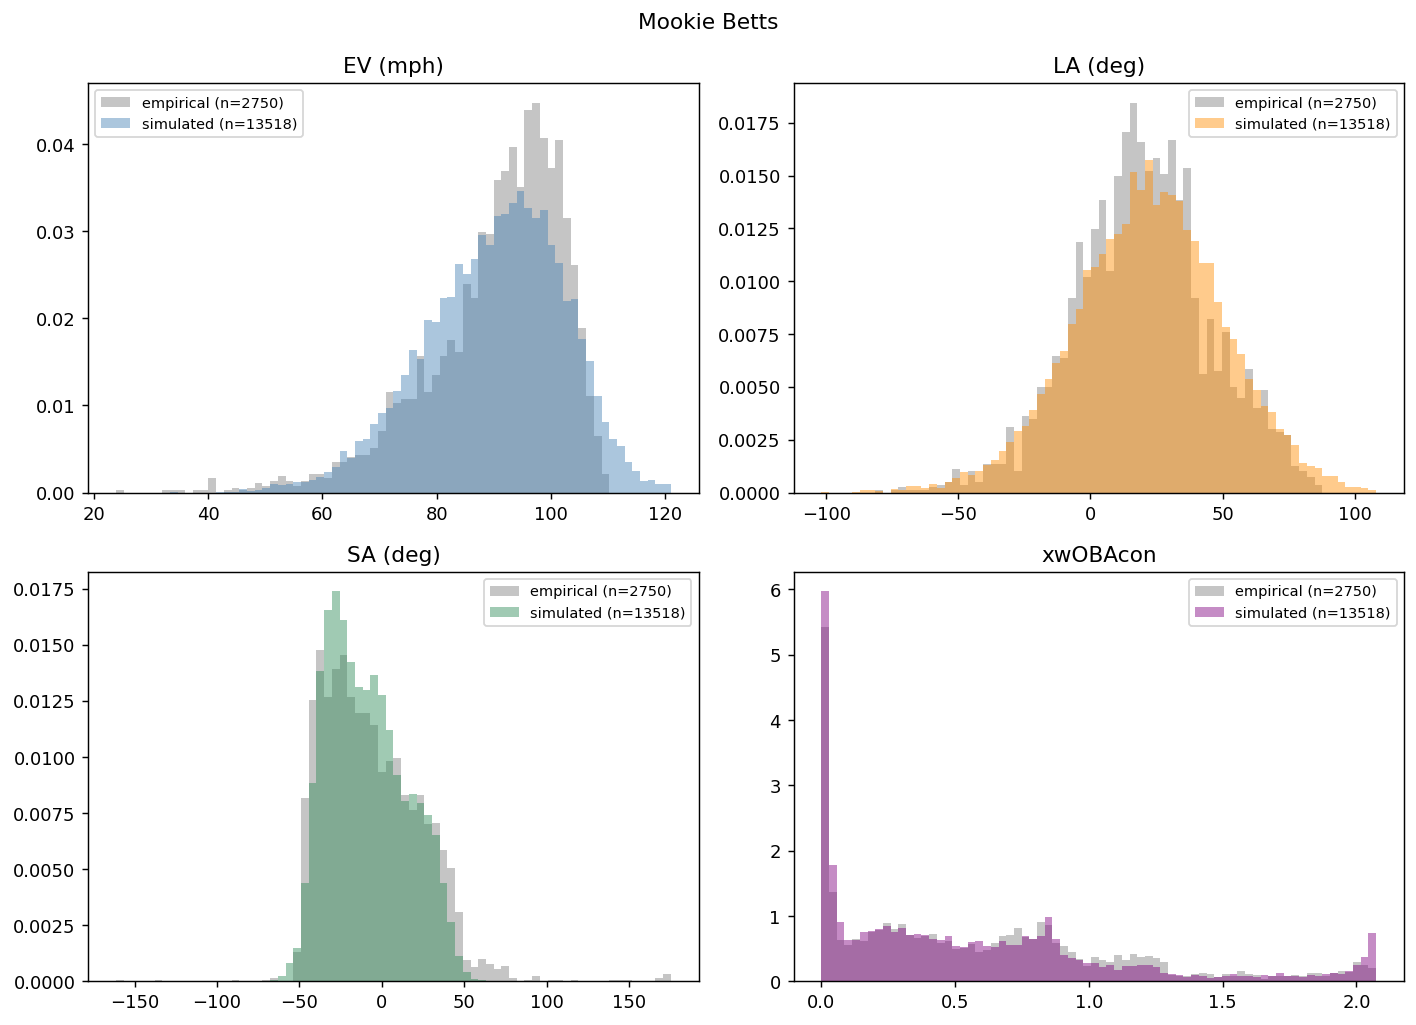
\includegraphics[width=\textwidth]{betts_overlay_empirical_vs_simulated_ev_la_sa_value.png}
    \caption{Simulated versus empirical distributional overlays for Mookie Betts. The four panels compare empirical and simulated distributions for exit velocity, launch angle, spray angle, and xwOBAcon. The simulated samples closely reproduce the central mass of the empirical exit velocity and launch angle distributions, while also capturing the broad structure of the spray angle distribution. The xwOBAcon panel provides a value-based diagnostic of the model's ability to reproduce the distribution of batted-ball quality after mapping simulated contact outcomes into expected offensive value. Overall, the overlay serves as a visual calibration check for whether the generative model produces realistic batted-ball outcomes for Mookie Betts across the primary physical and value-based output variables.}
    \label{fig:mookie_sim_emp_overlay}
\end{figure}



\subsection{Robustness Metrics}

\textbf{Pitch-Context Gaussian Mixture Model}

To evaluate hitter robustness across the pitch-design space, pitch contexts are grouped using Gaussian Mixture Models (GMMs). The purpose of the GMM is not to model batted-ball outcomes directly, but rather to define a set of representative pitch-context clusters from which the forward simulator can sample. Each sampled pitch context is then passed through the simulation model to generate a distribution of batted-ball outcomes.

Each pitch is represented by a seven-dimensional context vector,

\begin{equation}
    p_i
    =
    \begin{bmatrix}
        z_{\text{count},i} \\
        \text{plate\_x}_i \\
        \text{plate\_z}_i \\
        \text{release\_spin\_rate}_i \\
        \sin(\text{spin\_axis}_i) \\
        \cos(\text{spin\_axis}_i) \\
        \text{release\_speed}_i
    \end{bmatrix}
    \in \mathbb{R}^7 .
\end{equation}

Rather than fitting one global GMM with \(K = 57\), six separate GMMs are fit, one for each coarse pitch-type group. The total number of clusters is obtained by summing the manually selected component counts across groups:

\begin{center}
\begin{tabular}{c c c}
\hline
Pitch Group & Statcast Pitch Types & Number of Components \\
\hline
4F & FF, FA & 10 \\
2F & SI, FT & 9 \\
CF & FC & 8 \\
S  & SL, ST & 9 \\
C  & CU, KC, CS & 9 \\
CH & CH, FS & 12 \\
\hline
Total & -- & 57 \\
\hline
\end{tabular}
\end{center}

For each pitch group \(g\), the pitch-context vectors are standardized using a group-specific scaler. If \(S_g(\cdot)\) denotes this standardization map, then

\begin{equation}
    \tilde{p}_i
    =
    S_g(p_i).
\end{equation}

A diagonal-covariance GMM is then fit within each pitch group:

\begin{equation}
    q_g(\tilde{p})
    =
    \sum_{k=1}^{K_g}
    \pi_{g,k}
    \mathcal{N}
    \left(
        \tilde{p}
        \mid
        \mu_{g,k},
        \operatorname{diag}(\sigma^2_{g,k})
    \right),
\end{equation}

where \(K_g\) is the number of components assigned to pitch group \(g\), \(\pi_{g,k}\) is the mixture weight for component \(k\), \(\mu_{g,k}\) is the component mean, and \(\operatorname{diag}(\sigma^2_{g,k})\) is the diagonal covariance matrix.

The models are fit using expectation-maximization through \texttt{sklearn.mixture.GaussianMixture}. The fitting procedure uses diagonal covariance matrices, multiple random initializations, covariance regularization, and group-specific feature standardization. BIC/AIC grids are used only as diagnostic guidance; the production models use the fixed component map shown above.

After training, the six group-local GMMs are converted into a global set of 57 pitch clusters. Each pitch-context row is assigned to a local GMM component,

\begin{equation}
    \hat{k}_i
    =
    \arg\max_k
    \Pr(k \mid \tilde{p}_i, g),
\end{equation}

and the local component IDs are mapped into global cluster IDs \(c \in \{1,\dots,57\}\).

During robustness simulation, each global pitch cluster \(c\) corresponds to a specific pair \((g,k)\). New pitch contexts are sampled from that component:

\begin{equation}
    \tilde{p}^{(s)}_{g,k}
    \sim
    \mathcal{N}
    \left(
        \mu_{g,k},
        \operatorname{diag}(\sigma^2_{g,k})
    \right),
\end{equation}

and then transformed back into the original pitch-feature scale:

\begin{equation}
    p^{(s)}_{g,k}
    =
    S_g^{-1}
    \left(
        \tilde{p}^{(s)}_{g,k}
    \right).
\end{equation}

Each sampled pitch context is then passed into the forward simulator for hitter \(h\):

\begin{equation}
    p^{(s)}_{g,k}
    \longrightarrow
    (EV^{(s)}_{h,c}, LA^{(s)}_{h,c}, SA^{(s)}_{h,c})
    \longrightarrow
    V^{(s)}_{h,c},
\end{equation}

where

\begin{equation}
    V^{(s)}_{h,c}
    =
    xwOBAcon
    \left(
        EV^{(s)}_{h,c},
        LA^{(s)}_{h,c},
        SA^{(s)}_{h,c}
    \right).
\end{equation}

Thus, the GMM defines the pitch-context environments, while the physics-informed forward simulator defines the hitter's value distribution within each environment. The robustness metrics are then computed from the cluster-level value distributions. For hitter \(h\) and cluster \(c\), the cluster mean value is

\begin{equation}
    \mu_{h,c}
    =
    \frac{1}{N_{h,c}}
    \sum_{s=1}^{N_{h,c}}
    V^{(s)}_{h,c}.
\end{equation}

These cluster means are then used to compute the hitter's mean pitch value, pitch-type floor, and vulnerability gap. In this sense, the GMM provides the sampling structure needed to expose hitters to all regions of the pitch-design space, rather than only the pitch contexts they happened to face empirically.

\textbf{Cluster Mean Value}

For hitter \(h\), pitch cluster \(c\), and \(N_{h,c}\) simulated batted balls from that cluster, define the cluster mean value as

\begin{equation}
\mu_{h,c}
=
\frac{1}{N_{h,c}}
\sum_{j=1}^{N_{h,c}}
V_{h,c,j}.
\end{equation}

This represents the hitter's expected contact value against a specific pitch-design cluster.

\textbf{Mean Pitch Value Across Clusters}

If hitter \(h\) is evaluated across \(C_h\) pitch clusters, define the hitter's average pitch-cluster value as

\begin{equation}
\bar{\mu}_h
=
\frac{1}{C_h}
\sum_{c=1}^{C_h}
\mu_{h,c}.
\end{equation}

\begin{figure}[H]
    \centering
    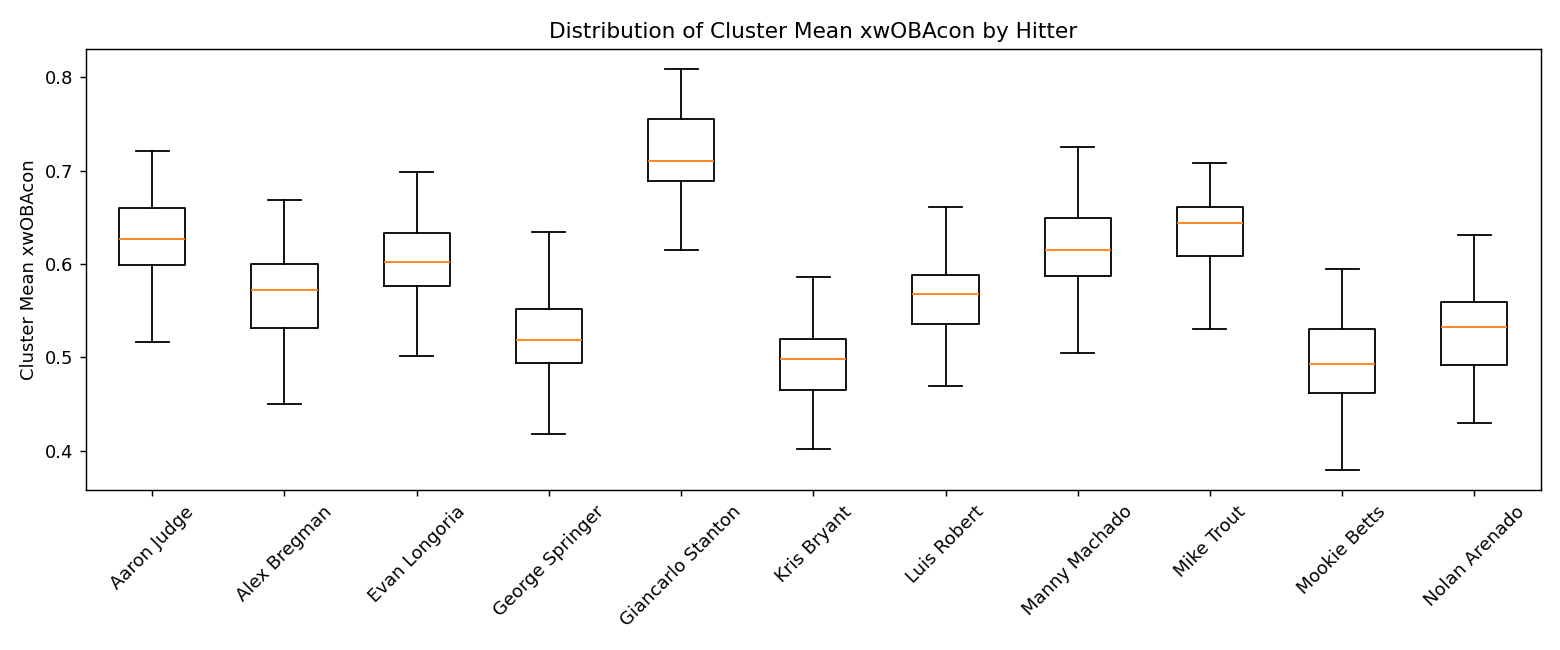
\includegraphics[width=\textwidth]{cluster_mean_distributions_boxplot.png}
    \caption{Distribution of cluster mean xwOBAcon by hitter. Each boxplot represents the distribution of simulated mean xwOBAcon values across pitch-type clusters for a given hitter. The median of each distribution reflects the hitter's typical cluster-level expected batted-ball value, while the spread captures variation in performance across different pitch contexts.}
    \label{fig:cluster_mean_xwobacon}
\end{figure}


Referring to figure 7, Giancarlo Stanton shows the highest cluster-level distribution, with a median well above the rest of the sample, suggesting strong simulated production across pitch-type groups. Mike Trout, Aaron Judge, Manny Machado, and Evan Longoria also show relatively high cluster-level value distributions. In contrast, Mookie Betts, Kris Bryant, and George Springer exhibit lower median cluster mean xwOBAcon values, implying weaker simulated production across the sampled pitch-type clusters.


This is the hitter's overall expected contact value across the full set of pitch-type clusters.

\textbf{Pitch-Type Robustness Score}

To measure downside robustness, sort hitter \(h\)'s pitch-cluster means from worst to best:

\begin{equation}
\mu_{h,(1)}
\leq
\mu_{h,(2)}
\leq
\cdots
\leq
\mu_{h,(C_h)}.
\end{equation}

Define the number of lower-tail clusters as

\begin{equation}
k_h
=
\left\lceil 0.10 C_h \right\rceil.
\end{equation}

The pitch-type robustness score, or lower-tail pitch floor, is

\begin{equation}
\operatorname{PitchFloor}_{h,10\%}
=
\frac{1}{k_h}
\sum_{i=1}^{k_h}
\mu_{h,(i)}.
\end{equation}

This measures the average value of the hitter's worst \(10\%\) of pitch-cluster matchups. A higher pitch floor indicates stronger downside robustness because the hitter remains productive even against his weakest pitch-design matchups.

\begin{figure}[H]
    \centering
    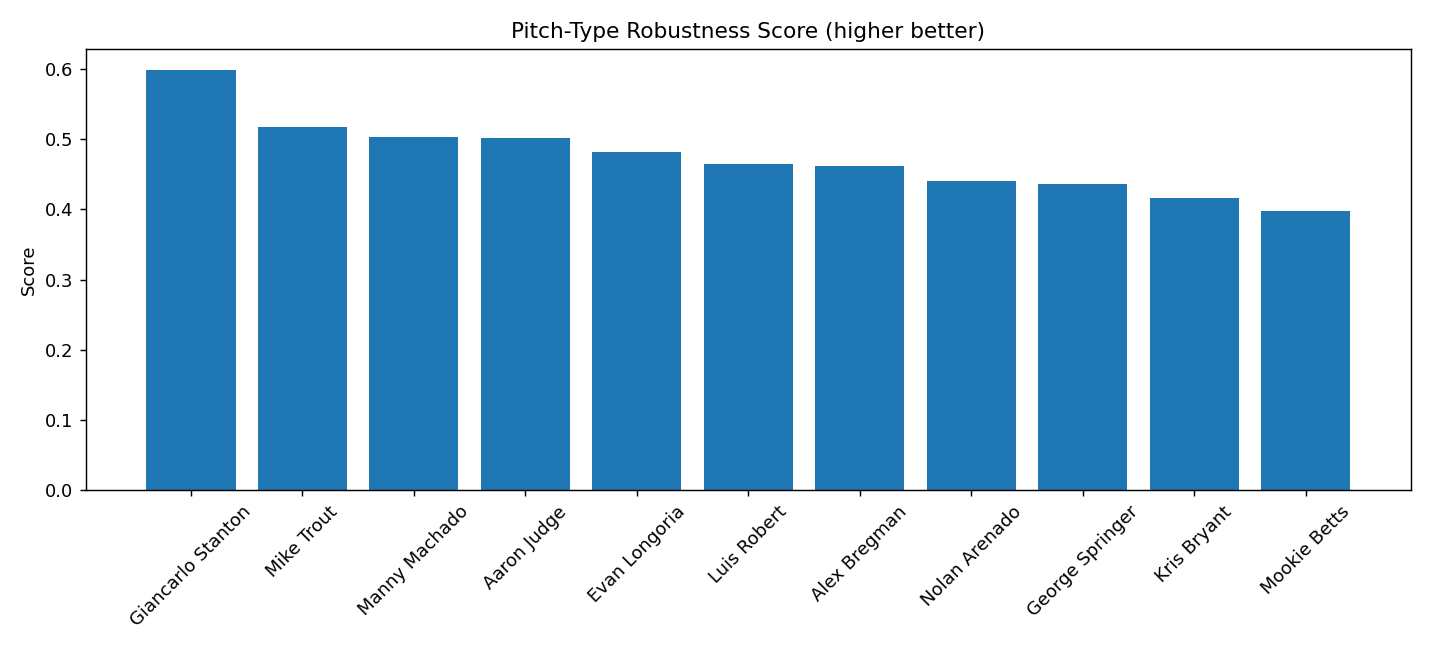
\includegraphics[width=\textwidth]{pitch_type_robustness_score_bar.png}
    \caption{Pitch-type robustness score by hitter. The robustness score summarizes how well a hitter maintains productive simulated batted-ball outcomes across the distribution of pitch-type clusters, with higher values corresponding to greater robustness. Giancarlo Stanton has the highest robustness score, followed by Mike Trout, Manny Machado, and Aaron Judge. This suggests that these hitters maintain stronger expected production across a broader range of pitch-type contexts. Mookie Betts, Kris Bryant, George Springer, and Nolan Arenado have lower robustness scores in this experiment, indicating comparatively weaker simulated production across the pitch-type cluster distribution.}
    \label{fig:pitch_type_robustness}
\end{figure}



\textbf{Vulnerability Gap}

The vulnerability gap compares the hitter's overall average pitch-cluster value to his lower-tail pitch floor:

\begin{equation}
\operatorname{VulnerabilityGap}_h
=
\bar{\mu}_h
-
\operatorname{PitchFloor}_{h,10\%}.
\end{equation}

A smaller vulnerability gap indicates that the hitter's downside profile remains close to his average value. A larger vulnerability gap indicates that the hitter may be neutralized by certain pitch designs.


```latex
\begin{figure}[H]
    \centering
    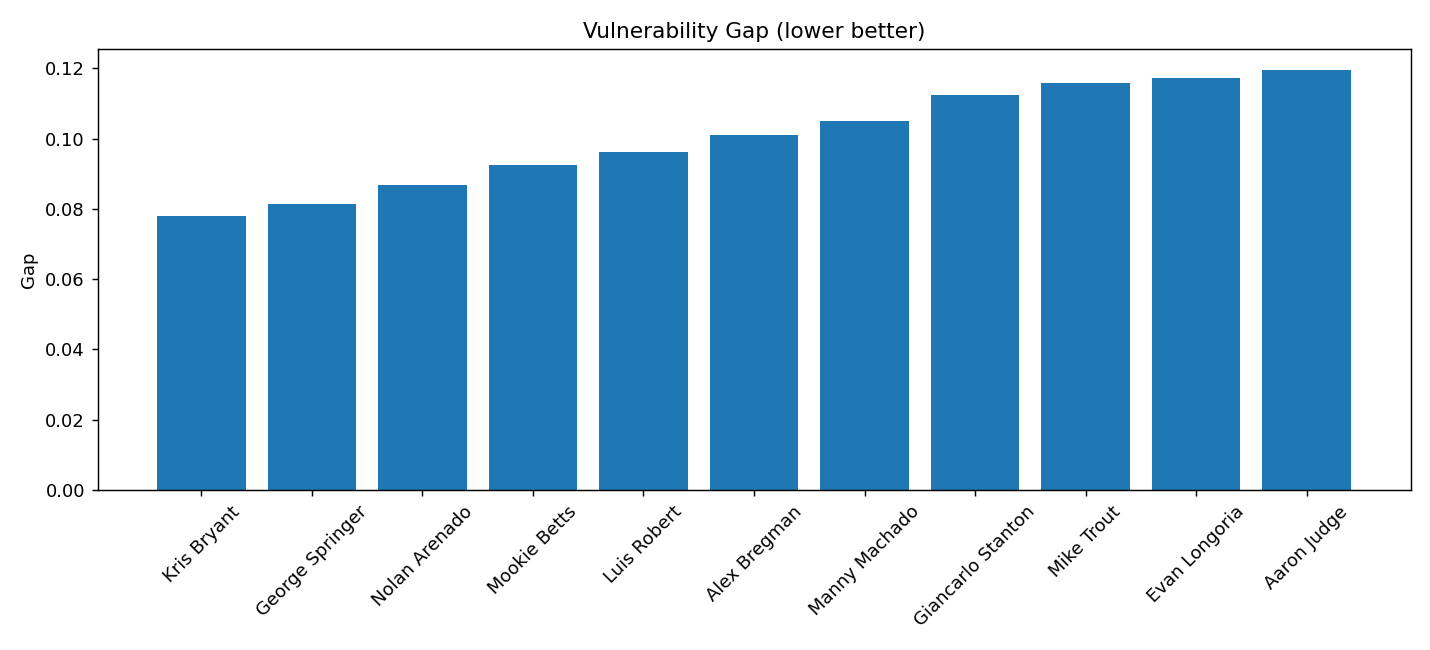
\includegraphics[width=\textwidth]{vulnerability_gap_bar.png}
    \caption{Vulnerability gap by hitter. The vulnerability gap measures the distance between a hitter's overall simulated batted-ball value and their lower-tail performance across pitch-type clusters. Lower values indicate that the hitter has a smaller drop-off against their weakest pitch-type contexts, while higher values indicate greater exposure to unfavorable pitch profiles. Kris Bryant, George Springer, and Nolan Arenado exhibit the lowest vulnerability gaps, suggesting more stable performance across pitch-type clusters. Aaron Judge, Evan Longoria, Mike Trout, and Giancarlo Stanton display larger vulnerability gaps, indicating that although these hitters may produce high average value, their performance is more sensitive to specific pitch-type contexts.}
    \label{fig:vulnerability_gap}
\end{figure}


\section{Counterfactual Case Study}

In the 2025 study done by Scott Powers and Ron Yurko, it was found that player's bat speed and bat length decreased as the number of strikes increased. From a straegic, intutive sense, it makes sense that batters would be more aggressive and "swing for the fences" in hitters counts, with less strikes, and take a more protective approach when they are deeper in the count or have a greater number of strikes against them.

We wanted to see if we could re-create this claim via simulation. This re-creation acts as a clear experiment as to if the generative model is actually learning causal mechanics and if it can recreate findings or at least the direction of findings of previous studies.

We organized the experiment as follows:

For each player, we simulated 5,000 pitches per count. In order to simulate a pitch, we sampled uniformly at random from the 57 pitch cluster GMM. After selection of a pitch type, we would sample from the corresponding GMM to generate the pitch context. We would then generate a swing for that player given the pitch context. For each player, they would have 20,000 pitches simulated per number of strikes. We then took the average bat speed for each number of strikes. The results are as follows:

\begin{table}[H]
\centering
\caption{Average Swing Speed by Strikes \\ \small{1000 simulations per count}}
\label{tab:avg_swing_speed_by_strikes}
\begin{tabular}{lccc}
\hline
\textbf{Player} & \textbf{0 Strikes} & \textbf{1 Strike} & \textbf{2 Strikes} \\
\hline
Aaron Judge      & 75.10 & 74.79 & 73.89 \\
Alex Bregman     & 70.16 & 69.93 & 69.34 \\
Evan Longoria    & 69.55 & 69.17 & 68.61 \\
George Springer  & 70.83 & 69.92 & 68.80 \\
Giancarlo Stanton& 80.28 & 79.70 & 79.12 \\
Kris Bryant      & 70.10 & 69.48 & 68.65 \\
Luis Robert      & 74.52 & 73.86 & 72.72 \\
Manny Machado    & 74.70 & 74.20 & 73.57 \\
Mike Trout       & 73.23 & 72.73 & 72.13 \\
Mookie Betts     & 68.53 & 68.31 & 67.60 \\
Nolan Arenado    & 71.28 & 70.76 & 69.59 \\
Pete Alonso      & 75.32 & 74.95 & 74.03 \\
\hline
\end{tabular}
\end{table}

As you can see, we were able to recreate directionally via generative modeling the results of Powers and Yurko that bat speed decreased as the number of strikes increased for all players. This directional replication of previous research serves as a checkpoint for a pitcher-hitter process generative model in testing the efficacy of the outputs generated from a counterfactual experiment.


\FloatBarrier

In general, the ability to ask counterfactual questions, organize experiments, and then run simulation to gain insights is a powerful tool. The previous case study acted as a "checkpoint" as to the efficacy of the generative model: Could it replicate previous studies? 

For this case study, we designed one of our own. We wanted to see if we can understand what the difference in Aaron Judge's swing for his best pitch cluster and his worst pitch cluster. Judge's best pitch cluster is a variation of a 4-seam fastball and his worst pitch cluster is a variation of a slider. The exact pitch context specifications are located in the appendix.

We ran 20,000 simulations from each of these pitch clusters and analyzed the distributions of where the ball made contact on the bat and the bat speed. We wanted to see if a difference in "squaring the ball up" or the bat speed of Judge caused the difference. There may be more variations of why EV could change, however these seemed like two plausible hypotheses which could cause EV to differ.

The impact location and bat speed distributions from simulation are shown below.

\begin{figure}[H]
    \centering
    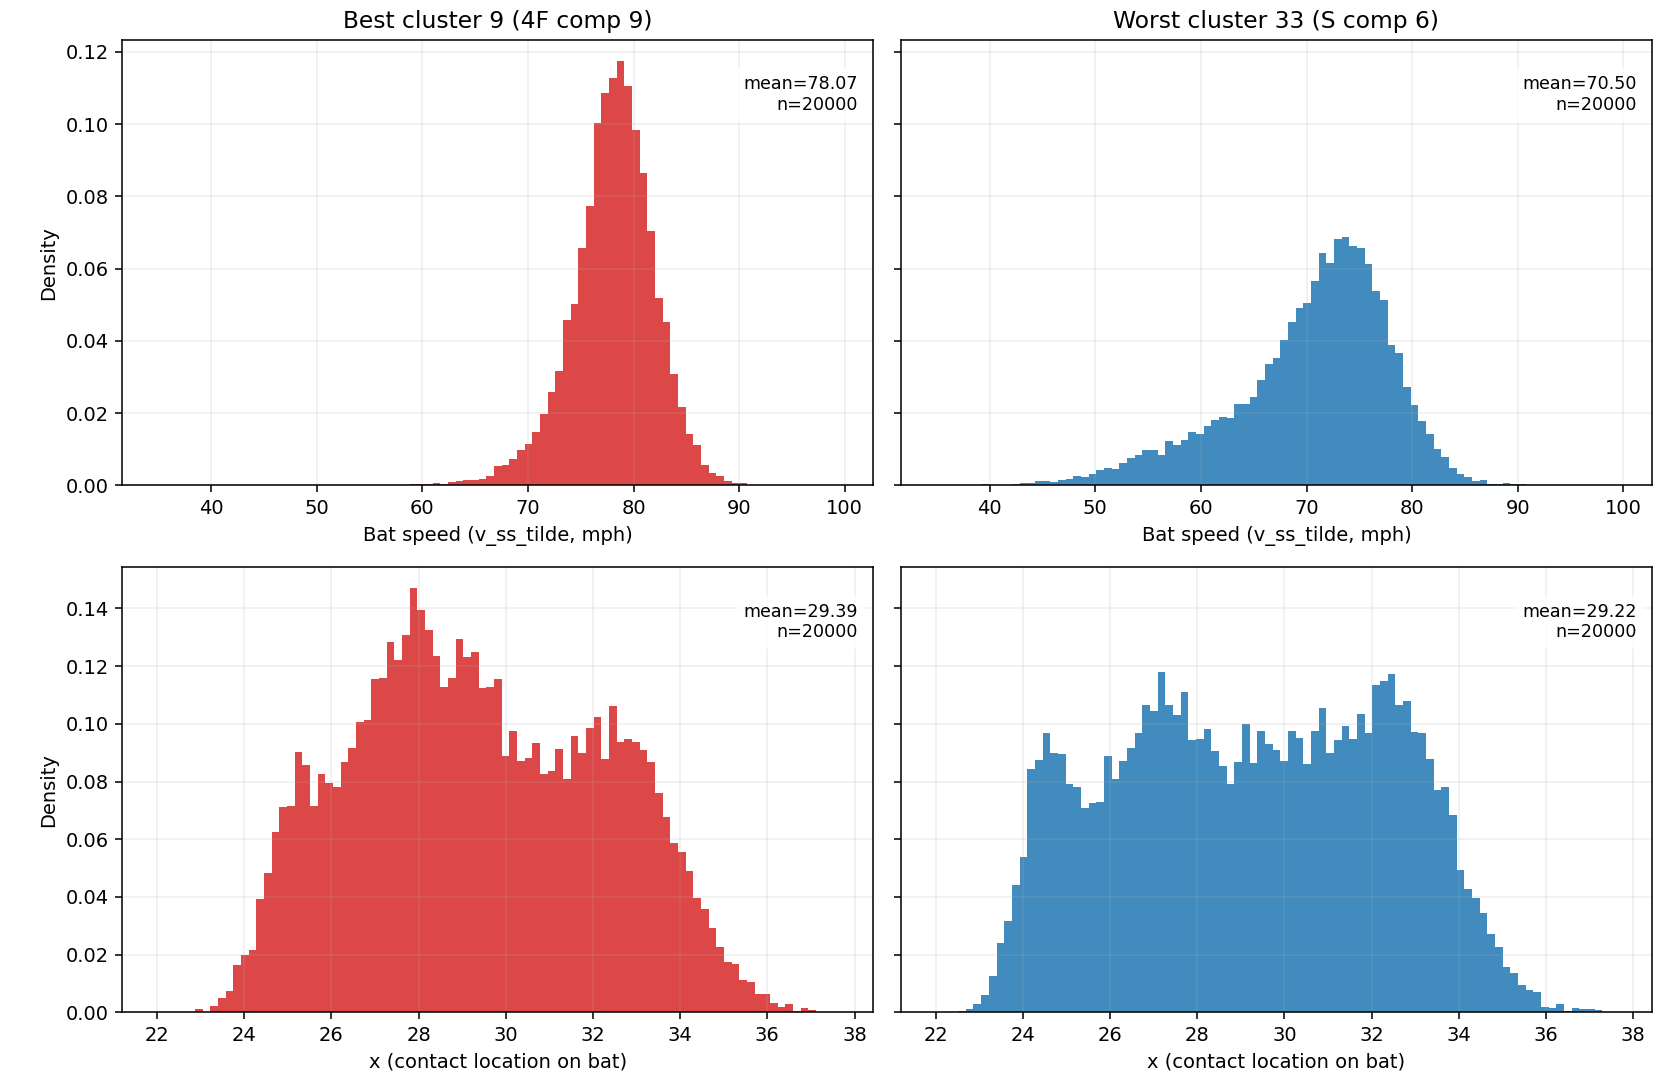
\includegraphics[width=\textwidth]{aaron_judge_cluster9_33_bat_speed_x_psi_20000_side_by_side.png}
    \caption{Comparison of simulated bat speed and contact-location distributions for Aaron Judge under his best and worst pitch-type clusters. The left column corresponds to the best-performing cluster, Cluster 9, labeled as a four-seam fastball component, while the right column corresponds to the worst-performing cluster, Cluster 33, labeled as a sinker component. The top row compares the simulated distribution of sweet-spot bat speed, \(v_{ss,\text{tilde}}\), while the bottom row compares the simulated distribution of contact location on the bat, \(x\). }
    \label{fig:judge_best_worst_cluster_batspeed_x}
\end{figure}

This simulation output shows that it isn't impact location but rather bat speed that creates the disparity in EV. The contact locations in the sweet spot interval [26,32] is actually very similar for both pitch clusters:

Cluster	% in interval
9 (best)
77.50%
33 (worst)
76.14%

However, there was a large discrepancy in the bat speed distributions where:

\begin{table}[H]
\centering
\caption{Bat Speed Percentiles for Aaron Judge's Best and Worst Pitch-Context Clusters}
\label{tab:judge_bat_speed_percentiles}
\begin{tabular}{lcc}
\hline
\textbf{Statistic} & \textbf{4-Seam Fastball (Best Cluster)} & \textbf{Slider (Worst Cluster)} \\
\hline
Mean              & 78.07 mph & 70.50 mph \\
10th percentile   & 73.21 mph & 59.82 mph \\
25th percentile   & 75.89 mph & 66.65 mph \\
75th percentile   & 80.60 mph & 75.63 mph \\
90th percentile   & 82.76 mph & 78.65 mph \\
\hline
\end{tabular}
\end{table}

Therefore we can conclude that for the Judge's worst slider context, using our mechanistic generative model, we show that Judge isn't producing lower exit velocities from mishits, but rather high bat-speed is considerably lower for this pitch cluster.

This counterfactual serves as a toy case study for just one of the many extensions of how generative models could help model and analyze the game of baseball beyond what empirical data can show us.

\section{Conclusion}

This study represents progress in applied machine learning in sports where physics, structure, and domain knowledge are heavily utilized to inform model architecture as opposed to letting ML learn the entire data-generating process unconstrained. It is shown that learning the data-generating process for a noisy, complex process rivals current "black-box" models and can even improve distributional prediction in the data sparsity regime. More work is needed to improve the model architecture for the pitcher-hitter process generative model in order to undrstand it's predictive ceiling compared to that of current black-box models.

We used these methodologies to augment the PyBaseball Statcast dataset to include all relevant collision variables in the data-generating process and sample those that were missing, built a generative model of the pitcher-hitter process, and then designed metrics that made use of the ability to simulate synthetic. The variance-adjusted metrics exposed distributional tendencies of hitters as opposed to pure expectation on the plate appearance level. While asymptotic performance over the long MLB season is important, consistency of performance at the PA level once a ball is put in play is also informative to a player's characterization and value. The robustness metrics aimed to encapsulate the gap between a player's average performance and their performance against the pitch types they perform most poorly against. The intuition here is that the larger the gap, the easier the hitter can be neutralized in high-leverage moments via pitch selection or pitching changes. 

\textbf{Future Directions}

In order to design the generative model of the pitcher-hitter process, we had to make many modeling and simplifying assumptions as to the nature of the process itself along with the statistical and machine learning methods used. While the modeling techniques we used worked well and the synthetic data closely resembles the data observed empirically, the modeling assumptions and choices made are by no means final or correct. A Mixture Density Network serves as a fair baseline, however Physics-Informed Neural Nets (PINNs) and Normalizing Flows among other model architectures serve as interesting possibilities in upgrading the generative model. 

Additionally, video data may be very useful in understanding the data-generating process at any even deeper level. While the constraints derived from experimentation and used in this study work well, it is plausible that that these constraints and relationships are not fully complete nor robust. Thus, deriving these physical relationships from video data could be important.

While we extended the ability to generate synthetic baseball data to constructing simulation-based metrics, there are many other use cases that can be thought of when it comes to generative models in baseball which include but are not limited to:

\begin{itemize}
    \item Lineup optimization
    \item Optimal pitch calling
    \item Offensive profile diversification
    \item In-game decision making, including pinch hitters and pitching changes
\end{itemize}

In addition, the ability to generate synthetic datasets opens up a range of possibilities within deep learning and reinforcement learning in sports.

Lastly, very broadly, the use of manifold embeddings for a given process in sports that exist in a broader ambient space is interesting. The thought of baseball and sports in general having certain geometric properties that may correspond to underlying structure is an interesting one. The same structure that leads to exit velocities forming a skew-normal distribution, may exist elsewhere, deeper in the system and process geometry. I leave this as an open thought for any researchers interested in diving further into the \textit{geometry of sports processes}.

\textbf{Closing Statements}

Correlation and patterns are insightful and hold real value for analysis and decision making, but the next step in the use of machine learning in sports may be towards generative models and simulation which encapsulate the mechanics and structure of how games unfold. For many systems or process this goal is currently out of reach, however for sports and especially baseball, the endeavor may be worthwhile. 

\newpage
\section{\textbf{Citations}}

\bibliographystyle{apalike}
\bibliography{references}


\newpage
\section{Appendix}

\subsection{Inverse-Collision Sampling Diagnostics}

The inverse-collision sampler should be interpreted primarily as a physics-constrained admissible-state sampler rather than as a conventional unconstrained posterior sampler. For fixed denoised measurement variables \(m^\star\) and normal restitution \(e_y^\star\), the bat-ball collision equations restrict the latent collision state
\[
\ell = (x,\psi,e_x,\omega^+)
\]
to a low-dimensional exact-root manifold embedded in the full latent space. Consequently, standard single-chain diagnostics such as acceptance rate, lag-1 autocorrelation, and effective sample size remain informative, but they do not fully characterize the success of the inverse procedure. In this setting, many rejected proposals correspond not to statistically inconvenient moves, but to mechanically impossible collision states.

The primary objective of the inverse stage is to recover latent collision configurations that satisfy the normal collision equation, tangential collision equation, spin update equation, measurement-error model, restitution support restrictions, tangential-regime restrictions, and all production admissibility checks. Therefore, finding admissible states is itself a nontrivial feasibility result. Across the production run, initialization and full-draw success were both approximately \(95.4\%\), indicating that the observed pre- and post-collision measurements usually admit at least one mechanically plausible latent explanation under the assumed collision model.

At the same time, the conventional MCMC diagnostics indicate weak local mixing, especially in the contact-location coordinate \(x\). The median acceptance rate was approximately \(2.1\%\), and the median effective sample size for \(x\) was approximately \(4.3\) retained draws. These diagnostics prevent us from interpreting the retained samples as fully converged independent posterior samples. Instead, the retained draws should be viewed as physically admissible inverse-collision samples, or as an empirical admissible-state target for downstream density estimation.

\begin{table}[H]
\centering
\caption{Production inverse-collision sampler diagnostics. Conventional MCMC diagnostics are reported alongside problem-specific feasibility and admissibility diagnostics because the target distribution is restricted by hard physical constraints.}
\begin{tabular}{p{0.28\textwidth} p{0.18\textwidth} p{0.44\textwidth}}
\hline
\textbf{Diagnostic} & \textbf{Result} & \textbf{Interpretation} \\
\hline
Initialization success & \(95.4\%\) & Most events admit at least one physically plausible latent collision state. \\
Full-draw success & \(95.4\%\) & Most events produced retained admissible latent-state samples. \\
Median proposal admissibility & \(5.0\%\) & Hard physical constraints reject most proposed states. \\
Median acceptance rate & \(2.1\%\) & Local Metropolis moves are sparse along the constrained support. \\
Median ESS for \(x\) & \(4.3\) & Local mixing in contact location is weak; retained samples are not independent posterior draws. \\
Median unique \(x\) values & \(13\) & Retained samples show some local diversity in contact location. \\
Median admissible \(x\)-intervals & \(1\) & Many events have simple, highly constrained contact-location support. \\
\hline
\end{tabular}
\end{table}

These diagnostics support a deliberately limited claim. The sampler should not be presented as producing gold-standard posterior samples for every event. Rather, it provides a large collection of mechanically admissible latent collision explanations that satisfy the imposed physics and measurement constraints. This distinction is important: weak local mixing limits posterior-mass interpretation, but it does not invalidate the feasibility result that the observed collisions can often be explained by physically plausible latent states under the model.


\subsection{Latent Collision Inference Priors}

We also place priors on the latent collision variables themselves. These priors encode physically plausible support before the exact-root collision equations and admissibility constraints are enforced.

\paragraph{Impact location.}
The impact location $x$ is the location of contact along the bat, measured from the knob toward the barrel. We restrict contact to the barrel region:
\[
x \sim \mathrm{Uniform}(L-11,L),
\]

This prior reflects the assumption that balls put in play are generated by contact on the hitting region of the bat rather than the handle or knob.

\paragraph{Normal coefficient of restitution.}
The normal coefficient of restitution is allowed to vary around the baseline effective restitution profile $e_y(x)$:
\[
e_y^{\ast}\mid x
\sim
\mathrm{TruncNormal}
\left(
e_y(x),\,
0.04^2,\,
[0.15,0.60]
\right).
\]
The truncation interval enforces physically plausible values. The mean function is constructed as a cubic spline from plot seen in (Nathan, 2003).

\paragraph{Tangential coefficient of restitution.}
The tangential coefficient of restitution $e_x$ is not sampled directly in the first proposal block. Instead, after the exact-root contact angle $\psi$ is found, $e_x$ is implied by the tangential collision equation. Its prior contribution is regime dependent:
\[
p(e_x\mid \mathrm{regime})
=
\begin{cases}
0,
&
\mathrm{gross\text{-}slip}, \\[4pt]
\mathcal{N}(e_x;0.4,0.1^2),
&
\mathrm{stick\text{-}slip}, \\[4pt]
\mathrm{Uniform}(0,0.6),
&
\mathrm{slip\text{-}stick\text{-}slip}.
\end{cases}
\]
The gross-slip regime is treated as inadmissible, while the remaining regimes encode physically plausible support for tangential energy transfer during oblique contact (Kelsrud, 2017).

Combining the measurement model and latent priors, the inverse-collision target density for an admissible state is
\[
\log \pi
\left(
x,m^{\ast},e_y^{\ast},\psi,e_x,\omega^{+}
\right)
=
\log p(x)
+
\log p(m^{\ast}\mid m^{\mathrm{obs}})
+
\log p(e_y^{\ast}\mid x)
+
\log p(e_x\mid \mathrm{regime}),
\]
with the collision equations and physical admissibility conditions enforced as hard constraints.


Since the observed exit speed s is treated as known in the inverse problem, the outgoing normal and tangential speeds are

\begin{equation}
V_n^+ = s \cos(\theta - \psi), \quad V_t^+ = s \sin(\theta - \psi).
\tag{10}
\end{equation}


\begin{table}[H]
\centering
\scriptsize
\begin{tabular}{llll}
\toprule
\textbf{Measured quantity} & \textbf{Code variable} & \textbf{$\sigma_j$} & \textbf{Rationale} \\
\midrule

Exit velocity $s$ &
\texttt{launch\_speed\_mph} &
$0.25$ mph &
Accounts for measurement error in observed exit speed. \\

Launch angle $\theta$ &
\texttt{launch\_angle\_deg} &
$0.50^\circ$ &
Allows uncertainty in the vertical batted-ball direction. \\

Hit coordinate $h_{c,x}$ &
\texttt{hc\_x} &
$0.75$ ft &
Propagates hit-location uncertainty into reconstructed spray angle. \\

Hit coordinate $h_{c,y}$ &
\texttt{hc\_y} &
$0.75$ ft &
Propagates hit-location uncertainty into reconstructed spray angle. \\

Bat speed $v_b$ &
\texttt{bat\_speed\_mph} &
$0.25$ mph &
Reflects uncertainty in measured bat speed entering contact kinematics. \\

Attack angle $a$ &
\texttt{attack\_angle\_deg} &
$0.50^\circ$ &
Allows uncertainty in the vertical swing-path angle. \\

Attack direction $d$ &
\texttt{attack\_direction\_deg} &
$0.75^\circ$ &
Allows uncertainty in the horizontal swing direction. \\

Initial pitch velocity $v_{x0}$ &
\texttt{vx0} &
$0.25$ ft/s &
Propagates pitch-trajectory uncertainty to contact. \\

Initial pitch velocity $v_{y0}$ &
\texttt{vy0} &
$0.25$ ft/s &
Propagates pitch-trajectory uncertainty to contact. \\

Initial pitch velocity $v_{z0}$ &
\texttt{vz0} &
$0.25$ ft/s &
Propagates pitch-trajectory uncertainty to contact. \\

Pitch acceleration $a_x$ &
\texttt{ax} &
$0.15$ ft/s$^2$ &
Accounts for uncertainty in reconstructed pitch acceleration. \\

Pitch acceleration $a_y$ &
\texttt{ay} &
$0.15$ ft/s$^2$ &
Accounts for uncertainty in reconstructed pitch acceleration. \\

Pitch acceleration $a_z$ &
\texttt{az} &
$0.15$ ft/s$^2$ &
Accounts for uncertainty in reconstructed pitch acceleration. \\

Release position $y_0$ &
\texttt{release\_pos\_y} &
$0.05$ ft &
Allows uncertainty in solving for pitch contact time. \\

Release spin rate $\omega_{\mathrm{spin}}$ &
\texttt{release\_spin\_rate\_rpm} &
$25.0$ rpm &
Reflects uncertainty in the spin magnitude used to construct pre-collision spin. \\

Spin axis $\gamma_{\mathrm{axis}}$ &
\texttt{spin\_axis\_deg} &
$1.0^\circ$ &
Allows uncertainty in the spin direction entering the tangential collision model. \\

\bottomrule
\end{tabular}
\caption{\footnotesize Production sensor-error scales used for the denoised observation block $m^{\ast}$ in the inverse-collision MCMC measurement model.}
\label{tab:mobs_sensor_priors}
\end{table}


\subsection{LightGBM Training for the xwOBAcon Value Mapping}



To estimate the probabilities in the xwOBAcon value function, we train a LightGBM multiclass classification model on historical batted-ball outcomes. The model does not directly regress on observed xwOBAcon. Instead, it learns the conditional outcome distribution

\begin{equation}
    \Pr(Y_i = o \mid EV_i, LA_i, SA_i),
    \qquad
    o \in \mathcal{O},
\end{equation}

where the outcome space is

\begin{equation}
    \mathcal{O}
    =
    \{Out, 1B, 2B, 3B, HR\}.
\end{equation}

Each batted-ball event \(i\) is represented by exit velocity, launch angle, and spray angle. Because spray angle is circular, it is encoded using sine and cosine transformations. Thus, the model input vector is

\begin{equation}
    x_i
    =
    \begin{bmatrix}
        EV_i \\
        LA_i \\
        \sin(SA_i) \\
        \cos(SA_i)
    \end{bmatrix}.
\end{equation}

The training target is the realized batted-ball outcome class,

\begin{equation}
    Y_i \in \{Out, 1B, 2B, 3B, HR\}.
\end{equation}

Singles, doubles, triples, and home runs are mapped directly into their corresponding classes. Field outs, force outs, double plays, sacrifice flies, and similar unsuccessful balls in play are mapped to the \(Out\) class. Events such as walks, strikeouts, hit-by-pitches, bunts, errors, and other non-standard batted-ball events are excluded so that the model is trained only on clean balls in play with observed \(EV\), \(LA\), and \(SA\).

The LightGBM model is trained as a multiclass classifier using the objective

\begin{equation}
    \mathcal{L}
    =
    -
    \sum_{i=1}^{N}
    \sum_{o \in \mathcal{O}}
    \mathbf{1}\{Y_i = o\}
    \log
    \hat{p}_o(x_i),
\end{equation}

where \(\hat{p}_o(x_i)\) is the model-implied probability that batted ball \(i\) belongs to outcome class \(o\). The model is trained using validation-set early stopping on multiclass log-loss. Class balancing is used to reduce the effect of outcome imbalance, especially for rare events such as triples.

After training, the raw LightGBM outputs are converted into class probabilities using the softmax function. A scalar temperature parameter \(T\) is fit on the validation set to improve probability calibration:

\begin{equation}
    \hat{p}_o^{\,cal}(x_i)
    =
    \frac{
        \exp\left(z_o(x_i)/T\right)
    }{
        \sum_{r \in \mathcal{O}}
        \exp\left(z_r(x_i)/T\right)
    },
\end{equation}

where \(z_o(x_i)\) is the raw model logit for outcome \(o\). This calibration step improves the reliability of the predicted probabilities before they are used in the value function.

The final xwOBAcon value is then computed as the expected linear-weight value of the calibrated outcome distribution:

\begin{equation}
    \widehat{xwOBAcon}_i
    =
    \sum_{o \in \mathcal{O}}
    w_o
    \hat{p}_o^{\,cal}(x_i).
\end{equation}

Since \(w_{Out}=0\), this becomes

\begin{equation}
    \widehat{xwOBAcon}_i
    =
    w_{1B}\hat{p}_{1B}^{\,cal}(x_i)
    +
    w_{2B}\hat{p}_{2B}^{\,cal}(x_i)
    +
    w_{3B}\hat{p}_{3B}^{\,cal}(x_i)
    +
    w_{HR}\hat{p}_{HR}^{\,cal}(x_i).
\end{equation}

Therefore, the LightGBM model provides a learned three-dimensional batted-ball value surface. Given a simulated batted-ball triple \((EV_i, LA_i, SA_i)\), the model returns the probability of each contact outcome, and xwOBAcon is computed as the weighted expectation of those outcome probabilities. In the robustness pipeline, this allows every simulated contact event to be mapped into a scalar value \(V_i\), which is then used to construct hitter-level pitch-cluster value distributions.

\begin{scriptsize}
\renewcommand{\arraystretch}{1.10}

\begin{longtable}{>{\raggedright\arraybackslash}p{0.24\textwidth}
                  >{\raggedright\arraybackslash}p{0.68\textwidth}}

\caption{Core physics variables for the bat--ball collision model.}
\label{tab:core_physics_variables} \\

\toprule
\textbf{Symbol} & \textbf{Definition} \\
\midrule
\endfirsthead

\toprule
\textbf{Symbol} & \textbf{Definition} \\
\midrule
\endhead

\bottomrule
\endlastfoot

\(\mathbf{c}_{\mathrm{bat}}\) 
& Center of the bat barrel at the point of contact. \\

\(\mathbf{c}_{\mathrm{ball}}\) 
& Center of the baseball at impact. \\

\(\hat{\mathbf{n}}\) 
& Unit normal direction at contact, pointing from the bat-barrel contact point toward the center of the baseball. \\

\(\hat{\mathbf{t}}\) 
& Unit tangential direction at contact, perpendicular to \(\hat{\mathbf{n}}\). \\

\(\hat{\mathbf{x}},\hat{\mathbf{y}},\hat{\mathbf{z}}\) 
& Global coordinate basis vectors. Positive \(x\) points toward first base, positive \(y\) points toward the pitcher, and positive \(z\) points upward. \\

\(\phi\) 
& Spray angle of the batted ball. This fixes the horizontal outgoing direction of the ball. \\

\(\theta\) 
& Launch angle of the batted ball. This fixes the vertical outgoing direction of the ball. \\

\(\psi\) 
& Contact angle defining the local collision basis under the coplanar assumption. \\

\(\hat{\mathbf{r}}(\phi)\) 
& Radial direction in the horizontal spray-angle plane. \\

\(\hat{\mathbf{c}}(\phi)\) 
& Horizontal direction orthogonal to \(\hat{\mathbf{r}}(\phi)\). \\

\(\hat{\mathbf{v}}_{\mathrm{out}}\) 
& Observed outgoing unit direction of the batted ball. \\

\(v_{\mathrm{exit}}\) 
& Exit speed of the batted ball. This replaces \(s\) and is equivalent to \(EV\). \\

\(x_{\mathrm{imp}}\) 
& Impact location along the bat, measured from the knob toward the barrel. This replaces bare \(x\). \\

\(x_{\mathrm{cm}}\) 
& Location of the bat center of mass along the bat axis. \\

\(b(x_{\mathrm{imp}})\) 
& Offset from the bat center of mass to the impact location, \(b(x_{\mathrm{imp}})=x_{\mathrm{imp}}-x_{\mathrm{cm}}\). \\

\(v_{B,n}^{-}\) 
& Pre-collision normal velocity component of the baseball. \\

\(v_{B,n}^{+}\) 
& Post-collision normal velocity component of the baseball. \\

\(v_{B,t}^{-}\) 
& Pre-collision tangential velocity component of the baseball. \\

\(v_{B,t}^{+}\) 
& Post-collision tangential velocity component of the baseball. \\

\(v_{b,n}^{-}\) 
& Pre-collision normal velocity component of the bat at the contact point. \\

\(v_{b,t}^{-}\) 
& Pre-collision tangential velocity component of the bat at the contact point. \\

\(\Delta_n\) 
& Pre-collision normal relative velocity between the bat and ball. \\

\(\Delta_t\) 
& Pre-collision tangential relative velocity between the bat and ball, including the spin-adjusted surface motion term when written in full. \\

\(\omega^{-}\) 
& Pre-collision spin component of the baseball relevant to tangential contact. \\

\(\omega^{+}\) 
& Post-collision spin component of the baseball after impact. \\

\(R_{\mathrm{ball}}\) 
& Radius of the baseball. This replaces bare \(r\). \\

\(R_{\mathrm{bat}}\) 
& Effective bat radius at the point of contact. This replaces bare \(R\). \\

\(D\) 
& Contact-geometry offset appearing in the spin-update equation. \\

\(e_n(x_{\mathrm{imp}})\) 
& Normal coefficient of restitution as a function of impact location. This replaces \(e_y(x)\). \\

\(e_n^{\ast}\) 
& Sampled or effective normal coefficient of restitution used in inverse-collision inference. This replaces \(e_y^{\ast}\). \\

\(e_t\) 
& Tangential coefficient of restitution. This replaces \(e_x\). \\

\(\alpha\) 
& Baseball inertia parameter used in the tangential collision and spin-update equations. \\

\(r_n(x_{\mathrm{imp}})\) 
& Effective normal recoil factor of the bat--ball system. This replaces \(r_y(x)\). \\

\(r_t(x_{\mathrm{imp}})\) 
& Effective tangential recoil factor of the bat--ball system. This replaces \(r_x(x)\). \\

\(m_{\mathrm{ball}}\) 
& Mass of the baseball. This replaces bare \(m\). \\

\(M_{\mathrm{bat}}\) 
& Mass of the bat. This replaces bare \(M\). \\

\(I_0\) 
& Bat moment of inertia about an axis through the center of mass. \\

\(I_z\) 
& Bat moment of inertia about the long axis of the bat. \\

\end{longtable}
\end{scriptsize}

\end{document}

